\chapter{Experimental Approach}
\section{Overview}
Software engineering is an ever-growing field that has seen significant advances in recent years. As software systems have become increasingly complex and critical to the functioning of modern society, the need for effective and efficient methods for designing, building, and maintaining software has become more pressing than ever. One of the key ways in which researchers in the field of empirical software engineering work to improve the state of the art is through experimental studies and analyses.

In this chapter we will present in detail the planning and approach we followed to establish the studies on the application of \tdd for \es developmnet, and analyze their results. 
A controlled experiment, the baseline, followed by its replication, was conducted with the participation of 9 undergraduate Master's degree and third-year Bachelor's degree computer science students enrolled in the \textit{Embedded Systems} course at the University of Salerno, in Italy. Participation in the studies was agreed upon by the students and was voluntary, with the outcome not directly affecting the final mark of the students for the exam; students were however awarded 2 bonus points on their final mark, in order to encourage their participation.
Before taking part in the first experiment, a set of lectures and training sessions was held with the objective of providing the participants with a body of knowledge on the topics tackled by the studies, namely unit testing, test scaffolding and the \tdd approach.

Afterwards, the participants were partitioned into two groups and tackled the first task of the baseline study, one group using \tdd, the other using \notdd; the task, \textit{IntelligentOffice} required the implementation of system responsible for handling various parameters and functionalities inside a smart office, including the detection of the workers, handling the lights and monitoring the CO2 levels inside the office.
For the second task, \textit{CleaningRobot}, the approach followed by the two groups was inverted, namely the group that implemented the first task using \tdd switched to \notdd and vice versa. This task concerned the development of an \es to manage a small cleaning robot, which had to move in a room to clean dust, while avoiding obstacles along the way.
After each task the participants were asked to fill a questionnaire to express their feelings about it.

For the replication study, the participants had to develop an additional task, this time at home on their own (\ie not under our supervision in a lab at the university), before submitting their implementation and deploying it on a real hardware platform, a \textit{Raspberry Pi Model 4}, and using real sensors and actuators. This task, \textit{SmartHome}, was focused on the implementation of an intelligent system which allowed for handling light, temperature, and gas levels inside a room.
Since the replication study was only made up of this task, the students were randomly assigned one of the two groups upon receiving the instructions for implementing this task.
The students were given a deadline to implement this project, and were asked to book a time slot, during which they would have deployed their implementation on hardware and would have tested it in real time by observing the behavior of the sensors and actuators; moreover, during each participant has been individually interviewed after the hardware deployment, in order to gather their feedback on the experiments.

Following the three tasks, we extracted the values for a set of predefined dependent variables by running the acceptance test suite we prepared for each task on the implementations delivered by the participants. These values, as well as the submitted post-questionnaires and final interview, were our primary subject of analysis to answer the established research questions on the impact of \tdd on the quality, production, and number of written test cases of the developers' implementation when tackling \ess.

Overall, this experimental study aims to contribute to the body of knowledge in the field of empirical software engineering by providing new insights and understanding into the application of \tdd for \es development.
Although the preliminary nature of our investigation, it has the merit to study for the first time the application of \tdd in a new development context, namely that of the \ess; therefore, our results can have several practical implications. For example, they could provide initial evidence on the application of TDD to the development of \ess so justifying future research on this matter and/or promoting or discouraging its adoption in an industrial setting.



\section{Research Questions}
As for the baseline experiment, and following the main research question presented in the introduction section of this thesis, we defined the main goal of this study by applying the Goal/Question/Metrics (GQM) template \cite{GQM}.
According to the GQM template, for an organization to measure purposefully it must first specify the goals for itself and its projects, then it must trace those goals to the data that are intended to define those goals operationally, and finally provide a framework for interpreting the data with respect to the stated goals.
\begin{framed}
\noindent
\textbf{Analyze} the use of \tdd 
\textbf{for the purpose of} evaluating its effects in the development of \ess
\textbf{with respect to} the internal and external quality of the developed \ess, the developers' productivity, and the number of written test cases
\textbf{from the point of} view of the researcher and lecturer 
\textbf{in the context of} an \es course involving second year Master's degree students in Computer Science.
\end{framed}

\noindent According to this objective, the following research questions were defined:
\begin{itemize}
    \item \textbf{RQ1.} Does the use of \tdd impact the external quality of the developed \es? And if so, to what extent?

    \noindent\textit{Aim}: The answer to this RQ has practical implications, especially within the Agile community. For example, in case the use of \tdd positively affects the external quality of \ess developed within implementation tasks, it would mean that it is the case to teach this development approach in academic contexts, with the ultimate goal of facilitating the adoption of this Agile development approach in the industry. That is, if the newcomers of the working market are familiar with TDD (because they learned and experienced it in the academic context), and it is shown that it produces better quality \ess, then the software industry could be encouraged to migrate their development from \notdd to \tdd.

    \item \textbf{RQ2.} Does the use of \tdd increase developers' productivity when developing \ess? And if so, to what extent?

    \noindent\textit{Aim}: A positive answer to this RQ has practical implications, since it would help us to further improve our body of knowledge in the context of \tdd applied to the development of \ess. For example, some software companies operating in the context of the development of \ess could be encouraged to use \tdd in case: \textit{(i)} there is evidence that this approach
    improves productivity and \textit{(ii)} developers are familiar with this approach before being hired (\eg \tdd has been learned at university).

    \item \textbf{RQ3.} Does the use of \tdd increase the number of test cases written by developers when developing \ess? And if so, to what extent?

    \noindent\textit{Aim}: 
\end{itemize}




\section{Participants}
The participants for the two experimental studies were computer science students at the University of Salerno, in Italy; they were a mix of second-year Master's degree students in Salerno, and students visiting the university by means of the Erasmus program; this last group was further made up of Master's degree students and third-year Bachelor's degree students. Both groups were enrolled in the \textit{Embedded Systems} course at the University of Salerno. As for the Master's students, not all of them had a computer science background (Bachelor's degree). Among the students taking the course, 9 participated. 

The study had both research and educational goals: on one hand, we conceived the study to answer our RQs; on the other hand, the study allowed the students to gain practical experience with \tdd applied to \ess. As for the educational goal, \tdd is a development approach widely used in several contexts \cite{DBLP:conf/esem/RomanoZBPS22}, and it seems to be promising in the development of \ess too \cite{TDDEC}.

Participating in the studies was voluntary: the students were informed that \textit{(i)} any gathered data would be treated anonymously and shared for research purposes only; \textit{(ii)} they could drop out of the study at any time if they wished to do so, and \textit{(iii)} they could achieve the highest mark in the course even if they didn't participate. Finally, as an incentive to encourage participation, those who took part in the studies were rewarded with 2 bonus points in their final mark for the course, in line with Carver \etal's advice \cite{DBLP:conf/metrics/CarverJMS03}.

Before the studies took place, we collected some information on the participants' knowledge and experience with programming and testing, in order to get a general idea of their personal preparation before the studies. To this end, the participants were asked to fill out a form in which they had to rate their experience using a Likert scale (where 1 means “very inexperienced” and 5 means “very experienced”). All the participants had programming experience and most of them rated such an experience as 3 out of 5 on the scale. 
As for testing, the participants were mostly not experienced with unit testing, since most of them chose 1 or 2 on their scale to represent their unit-testing experience; finally, three students had heard about \tdd, but none had had a practical experience with this technique before the study.

The participants for the experiments were later asked to carry out their task by either using \tdd or \notdd (\ie any approach they preferred, except for \tdd) depending on the group they were partitioned in, and on the period the task took place in. 





\section{Experimental tasks design}
The experimental objects designed for the studies are three code katas, \ie programming exercises aimed at practicing a technique or a programming language: in this case the design of a small \es. All three tasks were designed according to a target platform, a \textit{Raspberry Pi Model 4}, and using the \textit{Python} programming language. As for why this environment was chosen, compared to other programming languages and platforms typically used for \es or \iot projects (\eg \textit{Arduino} with \textit{C++}), in our opinion focusing on a higher level language such as \textit{Python} - which is still employed for \ess, either in its standard form or in its \textit{MicroPython} variant - allowed us to focus more on the implementation and logic details than we would have done by designing the tasks orbiting around lower level language features and mechanisms.
Furthermore, if we also take into account that some participants had a limited, mostly theoretical, knowledge of \ess prior to the course's end, we think that introducing these practical concepts with \textit{Python} made it easier for them to get a grasp on the main implementation concepts for \ess. Finally, participants relied on the \textit{PyCharm IDE} to implement all three tasks.

The target platform was considered even for the two tasks of the baseline study, which in the end did not have to be effectively deployed on hardware; this was done in order to make the mocked implementation of the participants resemble as closely as possible the embedded implementation. The main mocked component utilized was a facade for the \textit{Raspberry Pi}'s General Purpose Input/Output (GPIO) library, available as open source software on GitHub \cite{GPIOMock}. Other mocked components include third party libraries for some individual sensors and actuators, like for the \textit{DHT1} temperature and humidity sensor.
For the replication study, another factor that influenced the design of the code kata was the availability of the hardware, including sensors and actuators, as well as how hard these would have been to test in real time; for example, testing a gas sensor by actually releasing gas close to it  for extended period of times could be dangerous. For some sensors, on the other hand, this was not a concern since it was possible to manually trigger them by rotating an on-board potentiometer, effectively lowering or increasing the detection threshold for their respective measurements.

The replication project was deployed and tested inside a laboratory at the University of Salerno. Each participant had their project uploaded on the \textit{Raspberry Pi} board and \dots

For \textit{Exp1}, the experimental tasks were:
\begin{itemize}
    \item \textbf{\textit{IntelligentOffice}} (\textbf{IO}): 
    The sensors and actuators employed for this task are:

    \item \textbf{\textit{CleaningRobot}} (\textbf{CR}): as the name suggests, this task required participants to implement an \es to manage a small cleaning robot. This system received command strings from an external management unit, and had to move/rotate the robot inside the room accordingly, using two DC motors, one for the wheels, and one for the robot itself. Besides this, the robot had to be able to detect an obstacle in front of it by using an IR sensor, and had to communicate its position to the remote management system. Finally, an Intelligent Battery Sensor (IBS) was used to check the charge left of the internal battery of the robot, and a LED was turned on to signal the need for a recharge.
    while looking for obstacles and cleaning the dust along the way. 
\end{itemize}

As for \textit{Exp2}, the replication study, the task was the following:
\begin{itemize}
    \item \textbf{\textit{SmartHome}} (\textbf{SH}): 
\end{itemize}
Further details on the experimental objects, including user stories, hardware used, and other information, are provided as an appendix to this thesis.



\section{Study design}
The \textit{Embedded Systems} course, during which the study was conducted, started in September 2022 and covered the following topics: modeling and design of an \es, state machines, sensors and actuators, embedded processors, memory architectures, embedded security and privacy concepts, embedded operating systems and scheduling, and \es testing techniques.

As the pre-questionnaire for the study highlighted, few students had unit testing experience, and almost no participants ha dealt with \tdd up to that point. For this reason, these topics were covered through a series of frontal lectures and exercise/homework sessions in the weeks preceding the studies.

All the participants attended these lectures and training sessions during which they were trained on the main topics they would encounter during the future experimental tasks. The overall schedule for training sessions and studies was subdivided in the following days:
\begin{itemize}
    \item \textbf{D1.} Frontal lecture - Introduction on unit testing and its guidelines. Interactive exercise on unit testing.
    \item \textbf{D2.} Frontal lecture - Test scaffolding and \textit{Raspberry Pi}'s GPIO library. Interactive exercise on test scaffolding.
    \item \textbf{D3.} Frontal lecture - Introduction to Test-Driven Development. Interactive exercise on \tdd.
    \item \textbf{D4.} Training task - \tdd exercise and homework.
    \item \textbf{D6.} First experimental task for the baseline study - \textit{IntelligentOffice} (\textit{IO}).
    \item \textbf{D7.} Second experimental task for the baseline study - \textit{CleaningRobot} (\textit{CR}).
    \item \textbf{D8.} Start date for the replication study's task - \textit{SmartHome} (\textit{SH}).
\end{itemize}


The first task, \textit{IO} took place on Tuesday, December 6th 2022, while the second, \textit{CR} took place on Tuesday, December 13th 2022. 


The experimental design of our baseline study is an ABBA crossover \cite{DBLP:journals/tse/VegasAJ16}; it is a kind of within-participants design where each participant receives both treatments (\ie \textit{A} and \textit{B}). In ABBA crossover designs, there are two sequences (\ie \textit{G1} and \textit{G2}), defined as the order with which the treatments are administered to the participants, and two periods (\ie \textit{P1} and \textit{P2}), defined as the times at which each treatment is administered. The experimental groups correspond to the sequences. Also, to mitigate learning effects, each period is paired with a
different experimental task.

For the first period \textit{P1}, the group \textit{G1} was assigned the \tdd version of the first task, \textit{IntelligentOffice}, while the group \textit{G2} was assigned the \notdd version; on the other hand, during period \textit{P2}, the group \textit{G1} was assigned the \notdd version of the second task, \textit{CleaningRobot}, while the group \textit{G2} was assigned the \tdd version.
Therefore, at the end of the baseline study, every participant had tackled each experimental object only once.
As for the replication study, the group structure remained the same, however each participant was randomly assigned the \tdd or \notdd version of the third and final experimental task, \textit{SmartHome}. As a result, the design of this study is \textit{one-factor-with-two-treatments} \cite{DBLP:books/sp/WohlinRHOR00}, a kind of \textit{between-participants} design. The assignment of the participants for done randomly.

After each period of the controlled baseline study, participants were asked to fill out an online questionnaire, with the purpose of describing their general experience with the implementation of the task, focusing on their perceived complexity and testing approach. 
The structure of the post-questionnaires was made up of three interval scale questions, and a variable number of open-ended questions, two for the \tdd group and three for the \notdd group, with the latter having an additional question, as the first open-ended question, asking to provide information about the chosen approach for testing. Furthermore, the post-questionnaire presented at the end of period \textit{P2} contained an additional open-ended question: here, participants had to provide their feelings towards both testing practices, \tdd and \notdd, and compare them based on the two encountered tasks. 

\noindent More specifically, the interval scale questions were:
\begin{itemize}
    \item \textbf{Q1.} Regarding the comprehensibility of the provided user stories, I have found them: (Very unclear $|$ Unclear $|$ Neither clear nor unclear $|$ Clear $|$ Very clear).
    \item \textbf{Q2.} I have found the development task: (Very difficult $|$ Difficult $|$ Neither easy nor difficult $|$ Easy $|$ Very easy).
    \item \textbf{Q3.} Applying (\ie \tdd or \notdd) to accomplish the development task has been: (Very difficult $|$ Difficult $|$ Neither easy nor difficult $|$ Easy $|$ Very easy).
\end{itemize}

\noindent As for the open-ended questions, these were:
\begin{itemize}
    \item (\textbf{\notdd only}) Describe the no-TDD approach you have followed to accomplish the development task.
    \item Provide your feelings (both positive and negative) about (\ie \tdd or \notdd).
    \item Provide your feelings (both positive and negative) about the development task.
    \item (\textbf{Task 2 only}) After applying (\ie \tdd or \notdd) in the last exercise, do you have any thoughts on the differences between the two approaches and your preference for using one over the other?
\end{itemize}

\noindent Finally, no formal questionnaire was provided for the replication study; however, after the hardware deployment step, each participant was individually interviewed about their overall experience with the studies; the structure of the final interview was:
\begin{enumerate}
    \item Provide your feelings (both positive and negative) about the final development project, (\eg development pipeline, used technologies).
    \item Provide your feelings (both positive and negative) about the development approach (\ie \tdd or \notdd) used to accomplish the final development project:
        \begin{itemize}
            \item \tdd: did you perform any refactoring? 
            \item \notdd: did you test your implementation at all? If so, which approach did you use?
        \end{itemize}
    \item Provide your feelings about the overall training experience (seminars, exercises, and homework on \tdd and \notdd, experiments, and final task):
        \begin{itemize}
            \item Positive and negative points and challenges encountered when applying TDD
            \item What can be done to improve the application of TDD in the development of \ess
            \item Please provide a discussion on \tdd vs. \notdd in the development of \ess
        \end{itemize}
\end{enumerate}





\section{Independent and dependent variables}
The participants were asked to carry out each task by using either \tdd or the approach they preferred (\notdd), therefore one of the independent variables considered is \textbf{\textit{Condition}}, a nominal variable assuming two values, \tdd and \notdd. The data was collected over two periods for the controlled study, and over an additional period for the non-controlled study, so a second independent variable is \textbf{\textit{Period}}, assuming the values $P1, P2, and P3$. During the three periods both treatments (\tdd or \notdd) were applied. Finally, since the participants were split into two groups, the last independent variable is \textbf{Group}, which can assume the values \textit{G1} and \textit{G2}.


As for the dependent variables considered in the studies, these are: \textbf{\textit{QLTY}}, \textbf{\textit{PROD}}, \textbf{\textit{TEST}}, \textbf{\textit{CYC}}, \textbf{\textit{COG}}, \textbf{\textit{LOC}}.
The variables $QLTY$, $PROD$ and $TEST$ have been used in previous empirical studies on \noess \cite{DBLP:journals/tse/ErdogmusMT05}, \cite{DBLP:journals/tse/FucciETOJ17}, \cite{DBLP:conf/esem/Fucci0BCSTJ18}, \cite{DBLP:journals/ese/TosunDFVTESOTJJ17}. As for the others variables

QLTY quantifies the external quality of the solution a participant implemented. It is formally defined as follows: 
\[
    QLTY = \frac{\sum_{i=1}^{\#TUS} QLTY_i}{\#TUS} * 100 
\]
where $\#TUS$ is the number of user stories a participant tackled, while $QLTY_i$ is the external quality of the $i-th$ user story; to determine whether a user story was tackled or not, the asserts in the test suite corresponding to the story were checked: if at least one assert in the test suite for the story passed, than the story was considered as tackled. $\#TUS$ is formally defined as follows:
\[
    \#TUS = \sum_{i=1}^{n} 
        \begin{cases}
            1 & \text{$\#ASSERT_i(PASS) > 0$}\\
                0 & \text{otherwise}
        \end{cases}
\]
Finally, the quality of the $i-th$ user story (i.e., $QLTY_i$) is defined as the ratio of asserts passed for the acceptance suite of the $i-th$ user story over the total number of asserts in the acceptance suite for the same story. More formally:
\[
    QLTY_i = \frac{\#ASSERT_i(PASS)}{\#ASSERT_i(ALL)}
\]
As a result, the $QLTY$ measure deliberately excludes unattempted tasks and tasks with zero success; therefore, it represents a local measure of external quality calculated over the subset of user stories that the subject attempted. $QLTY$ is a ratio measure in the range $[0, 100]$.

PROD estimates the productivity of a participant. It is computed as follows:
\[
    PROD = \frac{\#ASSERT(PASS)}{\#ASSERT(ALL)} * 100
\]
where $ASSERT(PASS)$ is the total number of asserts that have passed, by considering all acceptance test suites, while $ASSERT(ALL)$ refers to the total number of asserts in the acceptance suites. The $PROD$ variable can assume values between 0 and 100, where a value close to 0 indicates low productivity in the implemented solution, while a value close to 1 refers to high productivity.

The $TEST$ variable quantifies the number of unit tests a participant wrote. It is defined as the number of assert statements in the test suite written by the participant; this variable ranges from 0 to $\infty$.


As for the additional three dependent variables, these were computed using SonarQube and provide additional insight regarding the quality in the implemented software solution, in terms of how hard the production code is to comprehend and therefore maintain. They can be defined as follows:
(\textbf{$CYC$}) refers to the Cyclomatic Complexity metric of the implemented solution; it is a value used to determine the stability and level of confidence in a program, and it measures the number of linearly-independent paths inside a program module. A program with a lower Cyclomatic Complexity is generally easier to understand and less "risky" to modify; it can be used as an estimate on how difficult the code will be to cover/test.

(\textbf{$COG$}) is the Cognitive Complexity of the solution; it is a measurement of how difficult a program module is to intuitively understand. A method's Cognitive Complexity is based on a few rules \cite{CognitiveComplexity}:
\begin{enumerate}
    \item Code is not considered more complex when it uses shorthand syntax that the language provides for collapsing multiple statements into one.
    \item Code is considered more complex for each "break in the linear flow of the code".
    \item Code is considered more complex when "flow breaking structures are nested"
\end{enumerate}

Finally, $LOC$ is the total number of lines of code written by the participant; it's defined as the sum of the individual lines of code in both the production code source file and the test code source file.

For both $CYC$ and $COG$ we only considered the production code, since there was no noticeable difference, besides one outlier, between the same metrics in the test files of the participants.

Generally speaking, the higher the values of $CYC$, $COG$, and $LOC$, the worse it is; software with high cyclomatic and cognitive complexity is more difficult to understand, maintain, and extend, and is more prone to errors and bugs. It is good practice to keep these complexities (as well as the number of lines of code, although to a lesser extent) as low as possible for easy maintenance and extendability.





\section{Analysis Methods}
\subsection{Individual analysis}
As a first way to examine the distribution of the dependent variables, we compute the descriptive statistics, for each of them (\ie $QLTY$, $PROD$, $TEST$, $CYC$, $COG$, and $LOC$). We organize this information inside a set of tables for each experimental task. Moreover, in order to provide a graphical representation of the data and to summarize the distributions, we employ box plot charts.

The information that can be extracted form a box plot chart includes:
\begin{itemize}
    \item \textbf{Minimum value}: the lowest value, excluding outliers (shown at the end of the lower whisker).
    \item \textbf{Maximum value}: the highest score, excluding outliers (shown at the end of the upper whisker).
    \item \textbf{Median}: marks the mid-point of the data and is shown by the line that divides the box into two parts. Half the values are greater than or equal to this value and half are less than this value.
    \item \textbf{Inter-quartile range}: the middle “box” represents the middle 50\% of values for the group. The range of values from lower to upper quartile is referred to as the inter-quartile range. The middle 50\% of scores fall within the inter-quartile range.
    \item \textbf{Upper quartile}: 75\% of the scores fall below the upper quartile.
    \item \textbf{Lower quartile}: 25\% of scores fall below the lower quartile.
    \item \textbf{Whiskers}: the upper and lower "whiskers" represent scores outside the middle 50\% (i.e. the lower 25\% of scores and the upper 25\% of scores).
    \item \textbf{Outliers}: observations that are numerically distant from the rest of the data. They are defined as data points that are located outside the whiskers of the box plot, and are represented by a dot.
\end{itemize}


\subsection{Aggregate analysis}
Meta-analysis is a statistical method used to combine the results of multiple studies in order to obtain a more precise estimate of the effect of the treatment/intervention. Its goal is to increase the power of the analysis and to provide a more robust estimate of the treatment effect.
There are different methods used to conduct a meta-analysis, but generally, the process involves identifying relevant studies, extracting data from them, and then analyzing the data using statistical techniques. The most common method of meta-analysis is the random-effects model, which accounts for between-study variation in addition to within-study variation.
In our case, we considered the Standard Mean Difference (SMD) as the measure of effect size for the meta-analysis. It represents the difference between two groups' mean values, standardized by dividing the difference by the standard deviation; SMD can be used to determine the overall effect size when comparing the results of the different studies. 

A forest plot is a common way to visually present the results of a meta-analysis: it is a representation of the effect estimates and their corresponding confidence intervals for each study included in the meta-analysis. The forest plot is divided into two parts: the left side shows the individual study results and the right side shows the overall effect estimate and its corresponding confidence interval.
In a forest plot, the SMD is often displayed as a diamond shape, with the width of the diamond representing the confidence interval of the estimate. The position of the diamond on the x-axis indicates the magnitude and direction of the effect size.
To read a forest plot chart, you need to understand the following elements:
\begin{itemize}
    \item Study name: This is the name of the study that is represented in the plot.
    \item Study size: This is the number of participants
    \item Effect estimate: This is the measure of the treatment effect for each study, typically shown as a point estimate (e.g. odds ratio, mean difference, relative risk)
    \item 95\% Confidence interval: this is the range of values within which the true effect is likely to lie, typically shown as a horizontal line. In a forest plot, it is  displayed as the horizontal line running through the diamond shape representing the SMD estimate.
\end{itemize}

In our case, we considered the baseline and replication as the two studies for the meta-analysis.



\subsection{Thematic analysis}
Thematic analysis is an approach widely used in qualitative psychology research to analyze data from interviews, focus groups, and other forms of open-ended data; this kind of analysis involves reading through the gathered unstructured data multiple times to identify recurrent patterns, concepts, or themes, and then coding these patterns using a set of codes or labels. The researcher then organizes the coded data into themes and sub-themes, which are then used to construct a narrative or report of the findings.

Template Analysis is a form of thematic analysis which emphasizes the use of hierarchical coding but balances a relatively high degree of structure in the process of analyzing textual data with the flexibility to adapt it to the needs of a particular study \cite{ThematicAnalysis}. In Template Analysis, it is permissible (though not obligatory) to start with some a priori themes, identified in advance as likely to be helpful and relevant to the analysis. These are always tentative, and may be redefined or removed if they do not prove to be useful for the analysis at hand.

In our study, we used thematic analysis to analyze the open-ended questions of the post-questionnaires for the two experimental tasks of the baseline experiment, as well as the individual participant interviews of the replication study.



\section{Results}
\subsection{Dependent variable analysis}
In this section we will report the values observed for each dependent variable during their individual analysis. For each experimental task, we will provide a table summarizing the minimum and maximum values, mean, median, and standard deviation of each dependent variable, for the two separate conditions (\ie \tdd and \notdd), before considering the values of the variable for the first two tasks simultaneously, in order to provide an overview of the differences between the two testing approaches.

Besides the tables, box plot charts will be used to visualize the values assumed by the dependent variables.
A box plot chart is a type of chart often used in explanatory data analysis; it visually shows the distribution of numerical data and skewness through displaying the data quartiles (or percentiles) and averages.

As we discussed in the dependent variables' definition section, in the end we did not take into account the cyclomatic and cognitive complexities of the test code written by the participants during the experimental tasks. 
Figure \ref{bp_task1_2_cyc_cog_test} shows the box plot chart for these metrics, relative to the experimental tasks for the baseline study:

\begin{figure}[htbp]
    \begin{subfigure}{0.5\textwidth}
        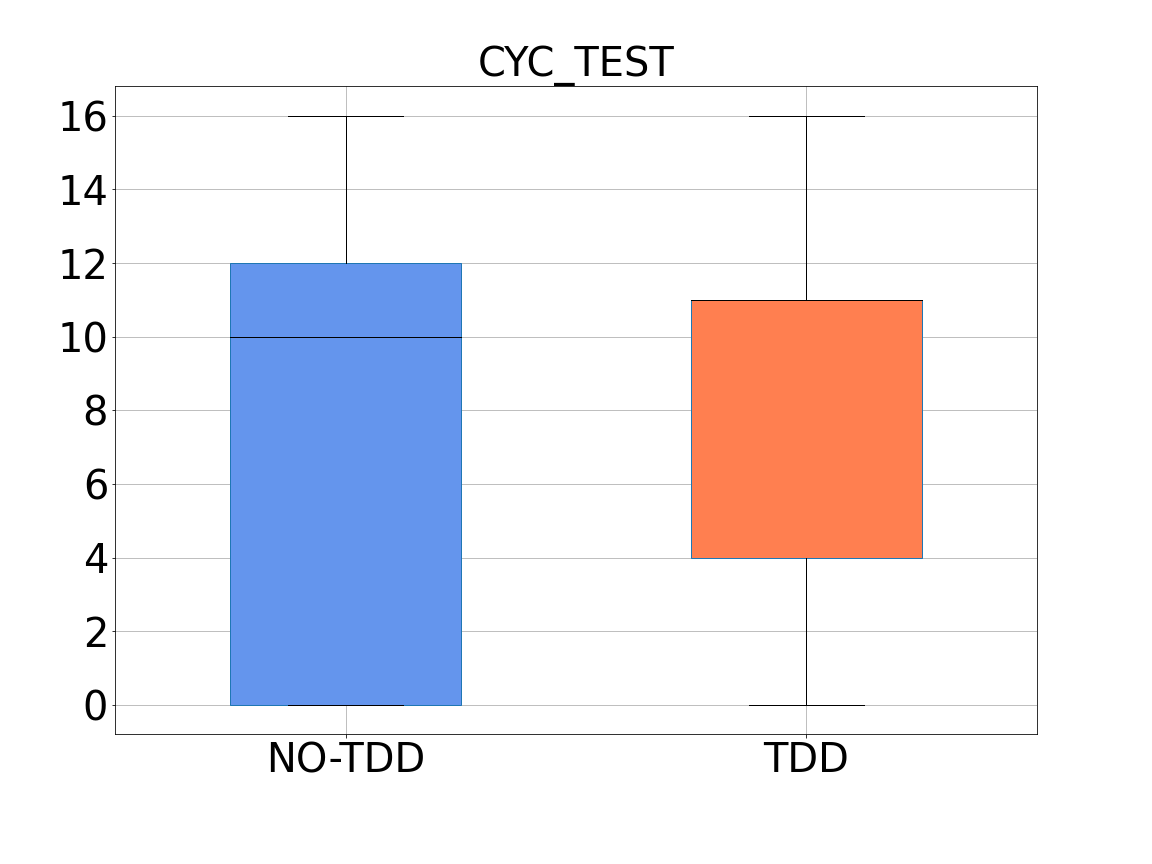
\includegraphics[width=\linewidth]{figures/box_plots/CYC_TEST.png}
        \caption{Cyclomatic complexity }
        \label{bp_task1_2_cyc_test}
    \end{subfigure}\hfil
    \begin{subfigure}{0.5\textwidth}
        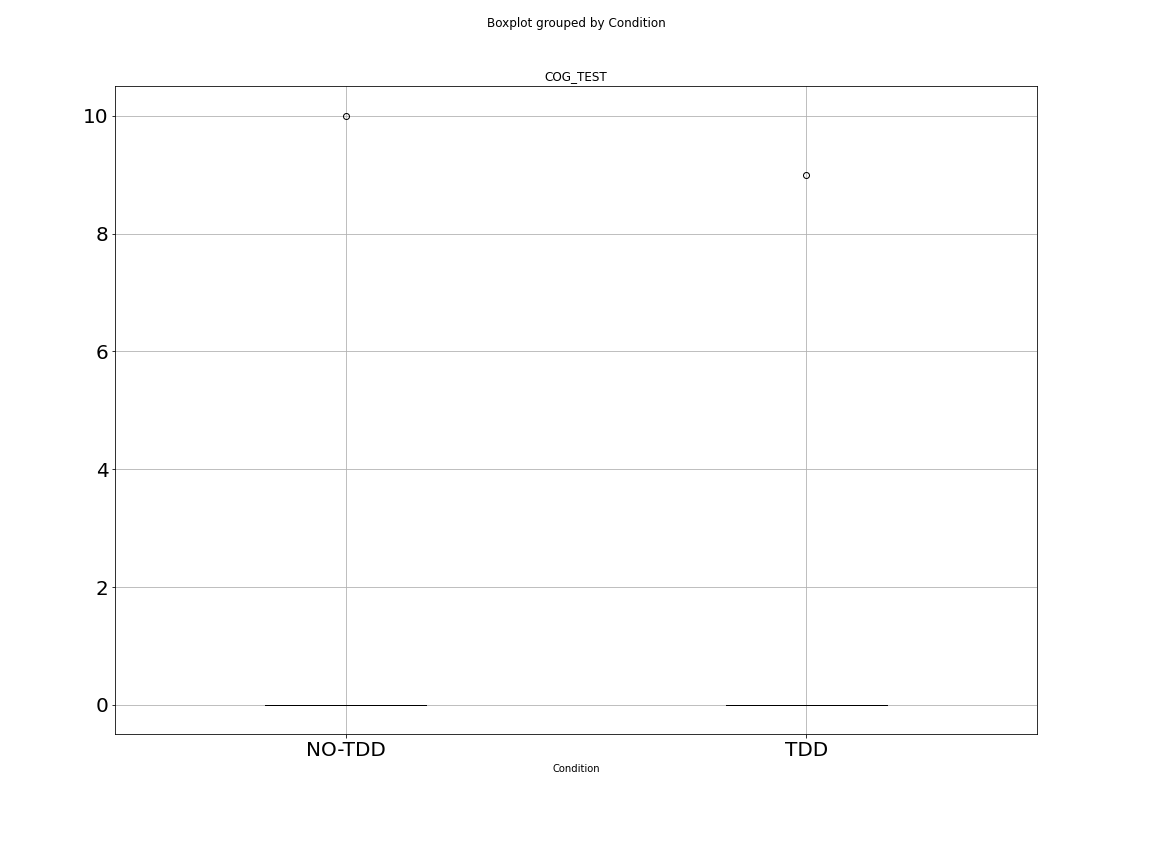
\includegraphics[width=\linewidth]{figures/box_plots/COG_TEST.png}
        \caption{Cognitive complexity}
        \label{bp_task1_2_cog_test}
    \end{subfigure}
    \caption{Box plots for the cyclomatic and cognitive complexities of test code for the first two tasks}
    \label{bp_task1_2_cyc_cog_test}
\end{figure}

Furthermore, we originally intended to also analyze the number of code smells in both the production and test code, however, as figure \ref{bp_task1_2_smells} highlights, there was no significant difference between the two conditions.

\begin{figure}[h]
    \centering
    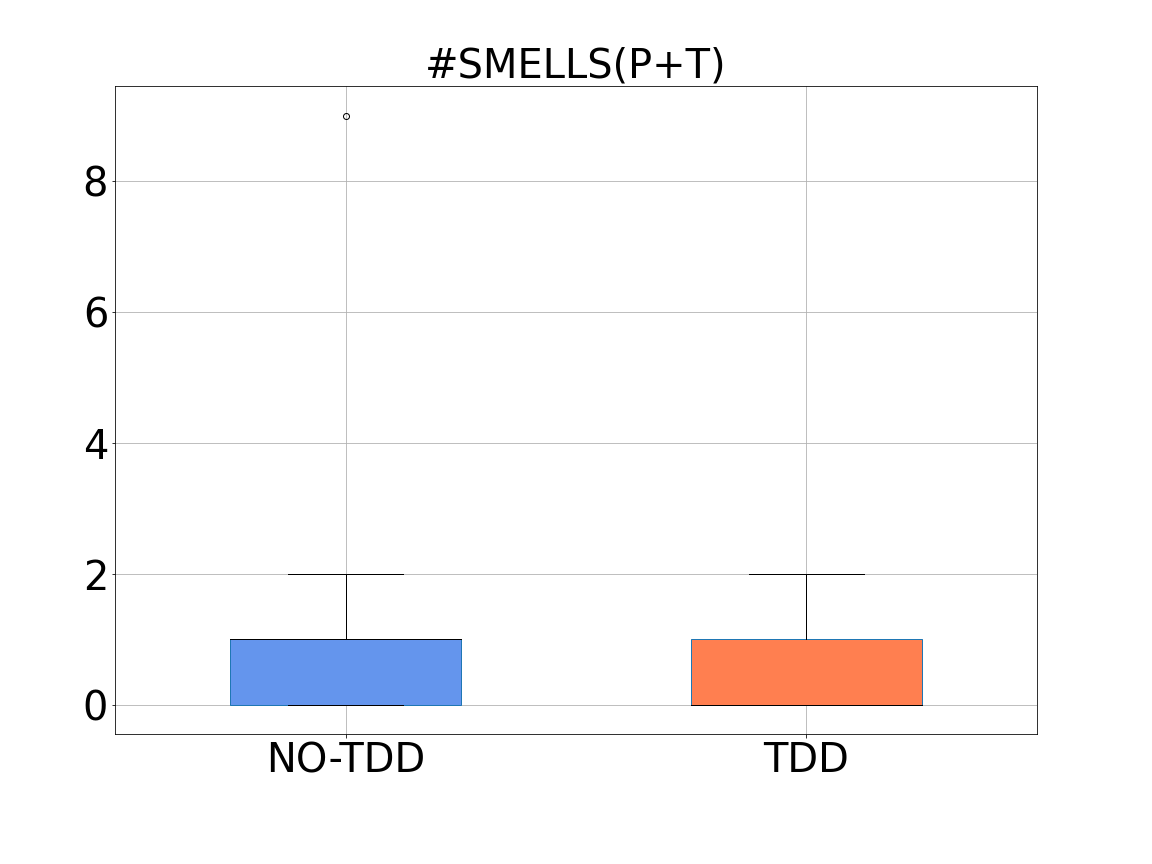
\includegraphics[width=0.5\linewidth, scale=0.5]{figures/box_plots/SMELLS.png}
    \caption{Number of code smells for the first two tasks}
    \label{bp_task1_2_smells}
\end{figure}


Starting with the first experimental task, tables \ref{tab_dv_t1_tdd} and \ref{tab_dv_t1_notdd}, as well as figure \ref{box_plots_task1} show the tables containing the extracted statistical measures and the box plot charts for the dependent variables, respectively.
$QLTY$ and $PROD$ paint a similar picture, with both having a similar median and values distribution among the two groups (standard deviations of 10 and 10.73, respectively), with the group employing \tdd reporting slightly higher average values.
As for the number of written tests, every participant in \textit{G1} (\tdd), except for an outlier, wrote a similar number of tests (\ie 9 or 10), with a standard deviation of only 1, compared to \textit{G2}, where the number of written test cases fluctuates a lot more; still, however, the median for \textit{G2} is 0, since a few participants did not write any tests at all.
The other code quality metrics, $CYC$, $COG$, and $LOC$ are on average higher for the \tdd implementations.

In task 2 (which, as emerged from the post-questionnaires, many participants found harder compared to the previous one), the \dots
(see \ref{tab_dv_t2_tdd} and \ref{tab_dv_t2_notdd}, and figure \ref{box_plots_task2}).
While the values for $QLTY$ are still higher for the \tdd group (\textit{G2} in this case), the same thing is not true for $PROD$; this suggests that among the participants that tackled the task using \tdd, there are some that only tackled the first user stories, and did so flawlessly, thus resulting in a high value for $QLTY$ (100\% median, and 84\% mean), and a lower value for $PROD$ (21\% median and 38.6\% mean). 
For the same reason, the average number of tests written is lower (5.4 average for \textit{G2} compared to the 9 average for \textit{G1}); the maximum value, however, is still higher for \textit{G2}, resulting from a participant correctly and fully applying \tdd to the task.

If we considered both tasks 1 and 2 simultaneously (see tables \ref{tab_dv_t1_2_tdd} and \ref{tab_dv_t1_2_notdd}, and figure \ref{box_plots_task1_2}).
$PROD$ has a much wider range of values for the \tdd group, given the result of task 2 and further highlighted by a standard deviation of 35, while for the \notdd group it is much more contained, ranging from 52\% to 84\%.

Finally, the task in the replication study (see tables \ref{tab_dv_t3_tdd} and \ref{tab_dv_t3_notdd}, and figure \ref{box_plots_task3}), produced results in favor of \tdd.
For the number of tests, we see a result in line with the first task, with the \tdd group producing on average more tests, and with the minimum values still well above the median of 3.5 for the \notdd group.
Regarding the code complexity metrics, ... . A higher value for $LOC$ is expected for the \tdd group since this metric contains both the lines of code written in the source files of the production code and the ones contained in the test code, so its value is directly related to the $TEST$ variable.

\begin{table}[!h]
    \begin{center} 
        \begin{tabular}{|p{1.8cm}||p{1.6cm}|p{1.6cm}|p{1.6cm}|p{1.6cm}|p{1.6cm}|p{1.6cm}|}
            \hline
                \multicolumn{6}{|c|}{Task 1 - TDD} \\
            \hline
                Metric & Min & Max & Mean & Median & Std \\
            \hline
                QLTY & 73 & 96 & 81.12 & 77.77 & 10.73 \\
                PROD & 72 & 96 & 83 & 82 & 10 \\
                TEST & 8 & 10 & 9.5 & 10 & 1 \\
                CYC & 21 & 28 & 24.75 & 25 & 2.87 \\
                COG & 14 & 25 & 19 & 18.5 & 4.69 \\
                LOC & 154 & 195 & 167 & 159.5 & 18.95 \\
            \hline
        \end{tabular}
        \caption{\label{tab_dv_t1_tdd}Dependent variables' statistics in task 1 for the \tdd group}
    \end{center}
\end{table}

\begin{table}[!h]
    \begin{center} 
        \begin{tabular}{|p{1.8cm}||p{1.6cm}|p{1.6cm}|p{1.6cm}|p{1.6cm}|p{1.6cm}|}
            \hline
                \multicolumn{6}{|c|}{Task 1 - NO-TDD} \\
            \hline
                Metric & Min & Max & Mean & Median & Std\\
            \hline
                QLTY & 65.55 & 82 & 75.35 & 78.77 & 7.43 \\
                PROD & 56 & 84 & 76 & 80 & 11.66 \\
                TEST & 0 & 12 & 3.8 & 0 & 5.49 \\
                CYC & 12 & 18 & 15.6 & 16 & 2.19 \\
                COG & 9 & 17 & 14 & 15 & 3 \\
                LOC & 74 & 157 & 111.6 & 100 & 33.69 \\
            \hline
        \end{tabular}
        \caption{\label{tab_dv_t1_notdd}Dependent variables' statistics in task 1 for the \notdd group}
    \end{center}
\end{table}

\begin{figure}[htbp]
    \centering
    \begin{subfigure}{0.33\textwidth}
        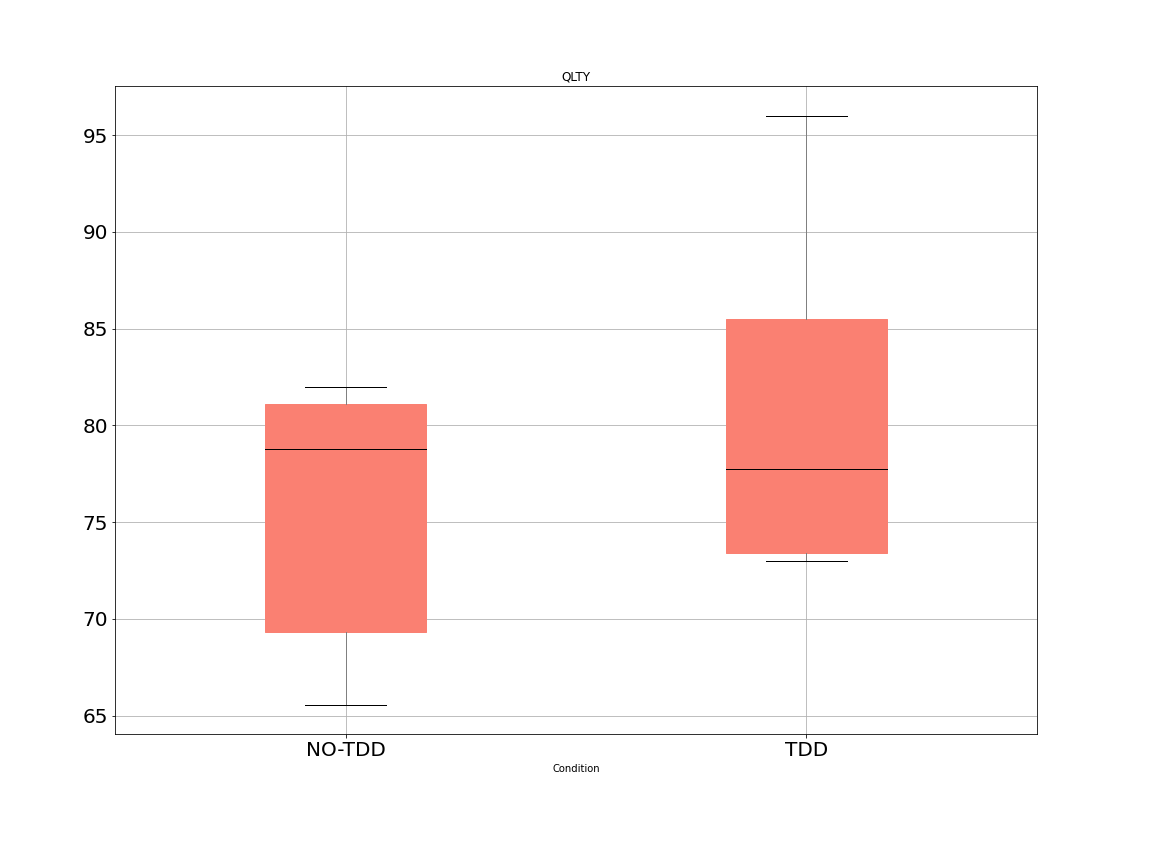
\includegraphics[width=\linewidth]{figures/box_plots/task1/QLTY.png}
        \caption{QLTY}
        \label{bp_task1_qlty}
    \end{subfigure}\hfil
        \begin{subfigure}{0.33\textwidth}
        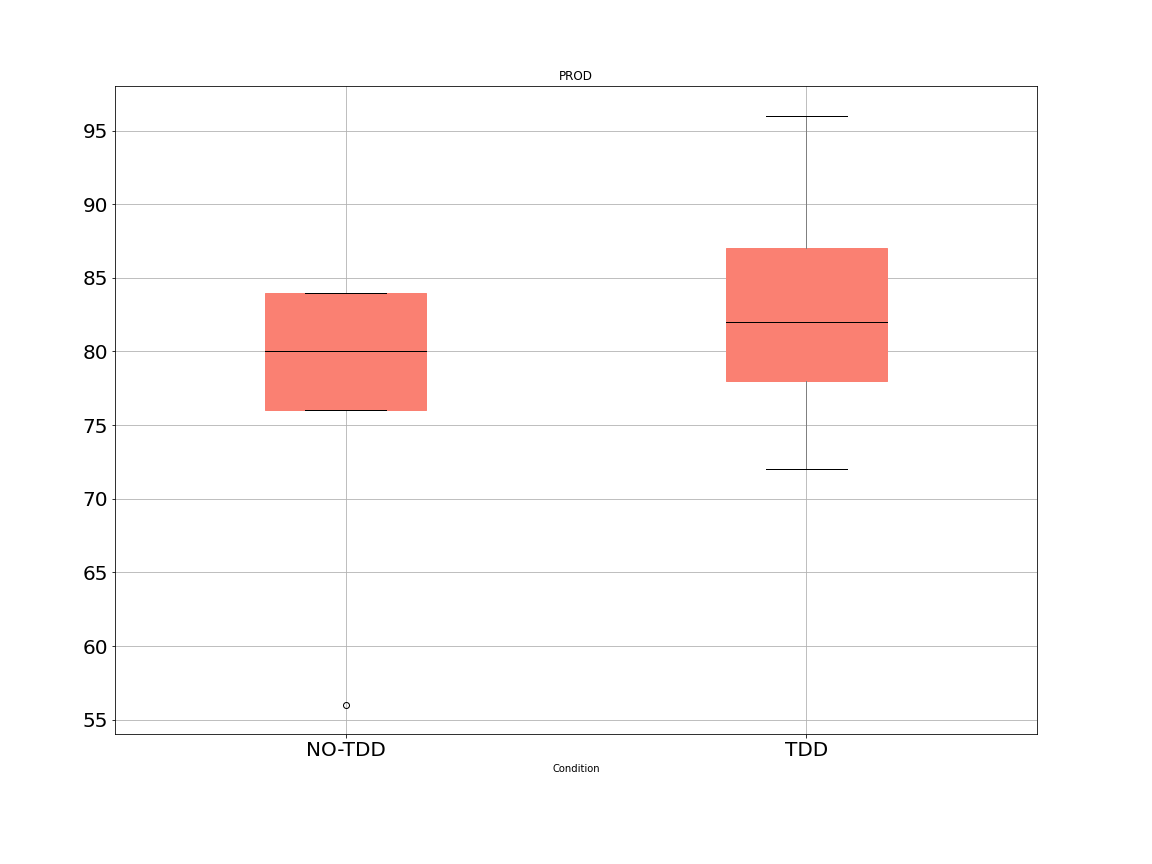
\includegraphics[width=\linewidth]{figures/box_plots/task1/PROD.png}
        \caption{PROD}
        \label{bp_task1_prod}
    \end{subfigure}\hfil
    \begin{subfigure}{0.33\textwidth}
        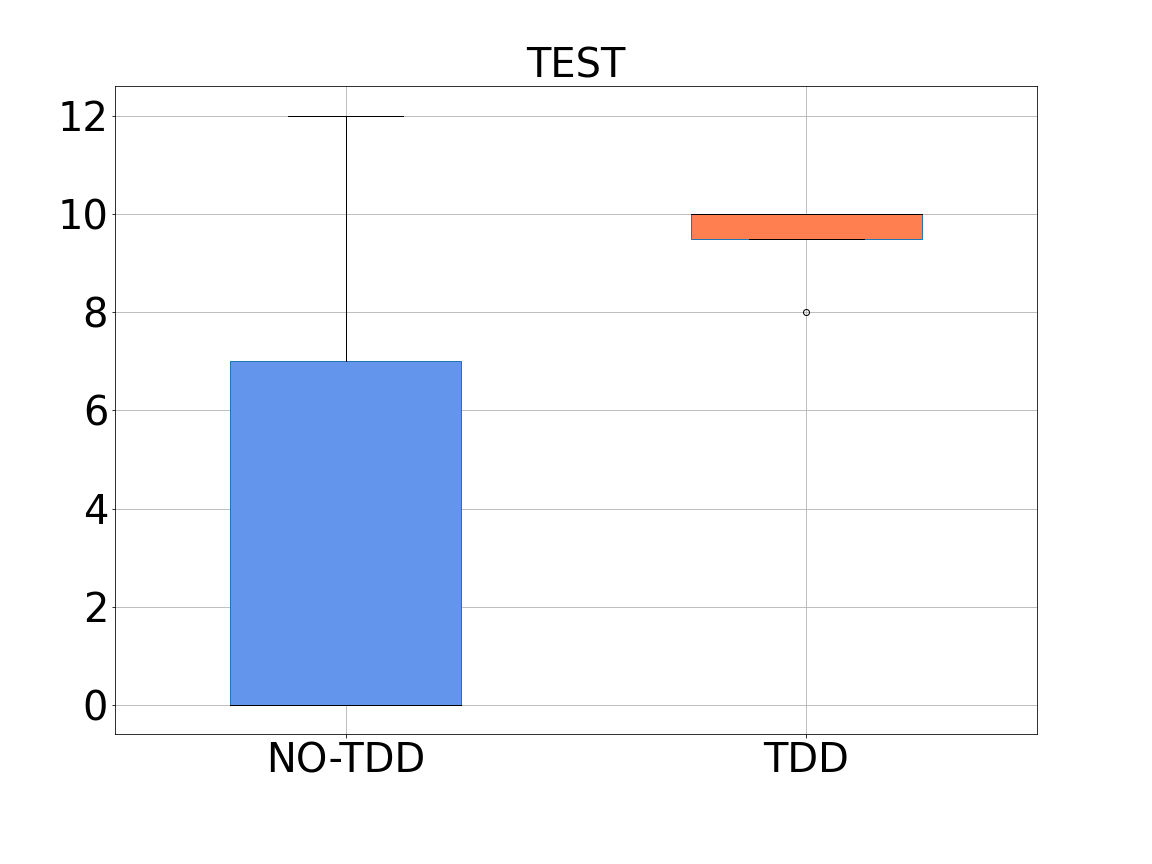
\includegraphics[width=\linewidth]{figures/box_plots/task1/TEST.png}
        \caption{TEST}
        \label{bp_task1_test}
    \end{subfigure}

    \medskip
    \begin{subfigure}{0.33\textwidth}
        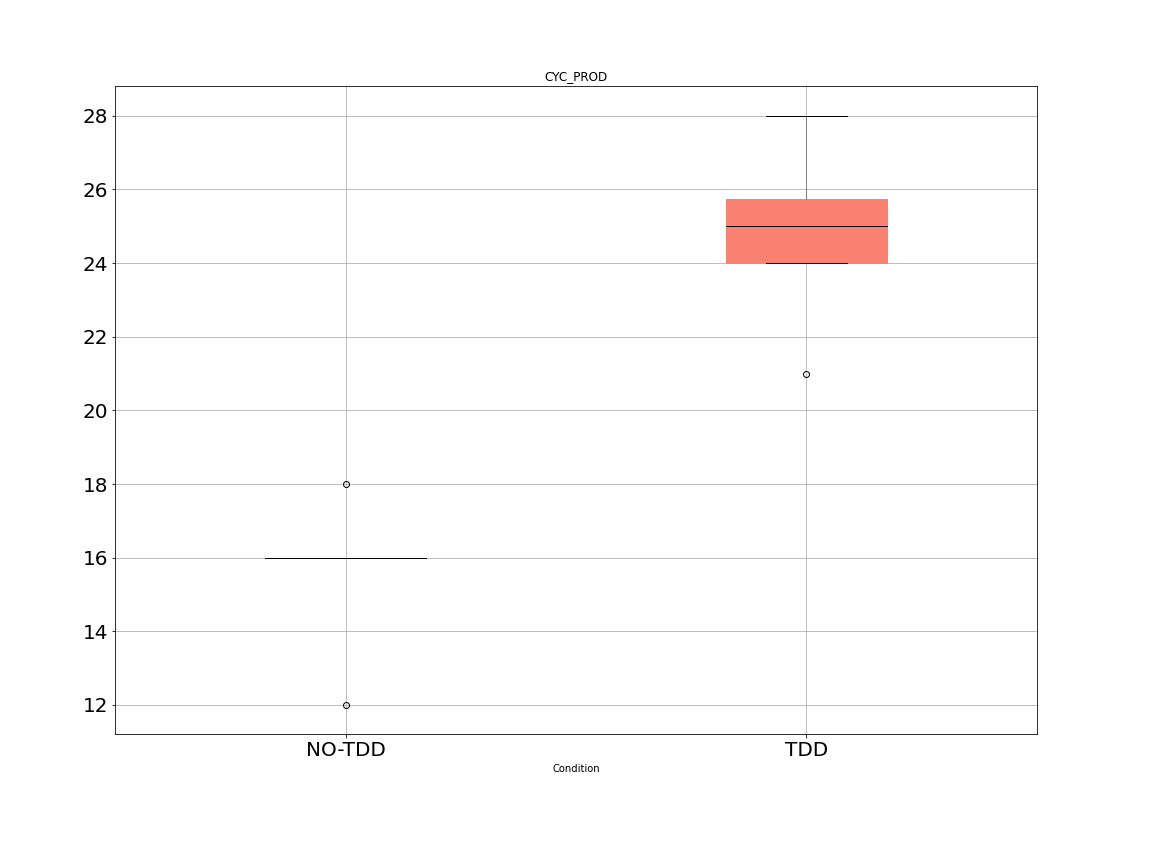
\includegraphics[width=\linewidth]{figures/box_plots/task1/CYC.png}
        \caption{CYC}
        \label{bp_task1_cyc}
    \end{subfigure}\hfil
    \begin{subfigure}{0.33\textwidth}
        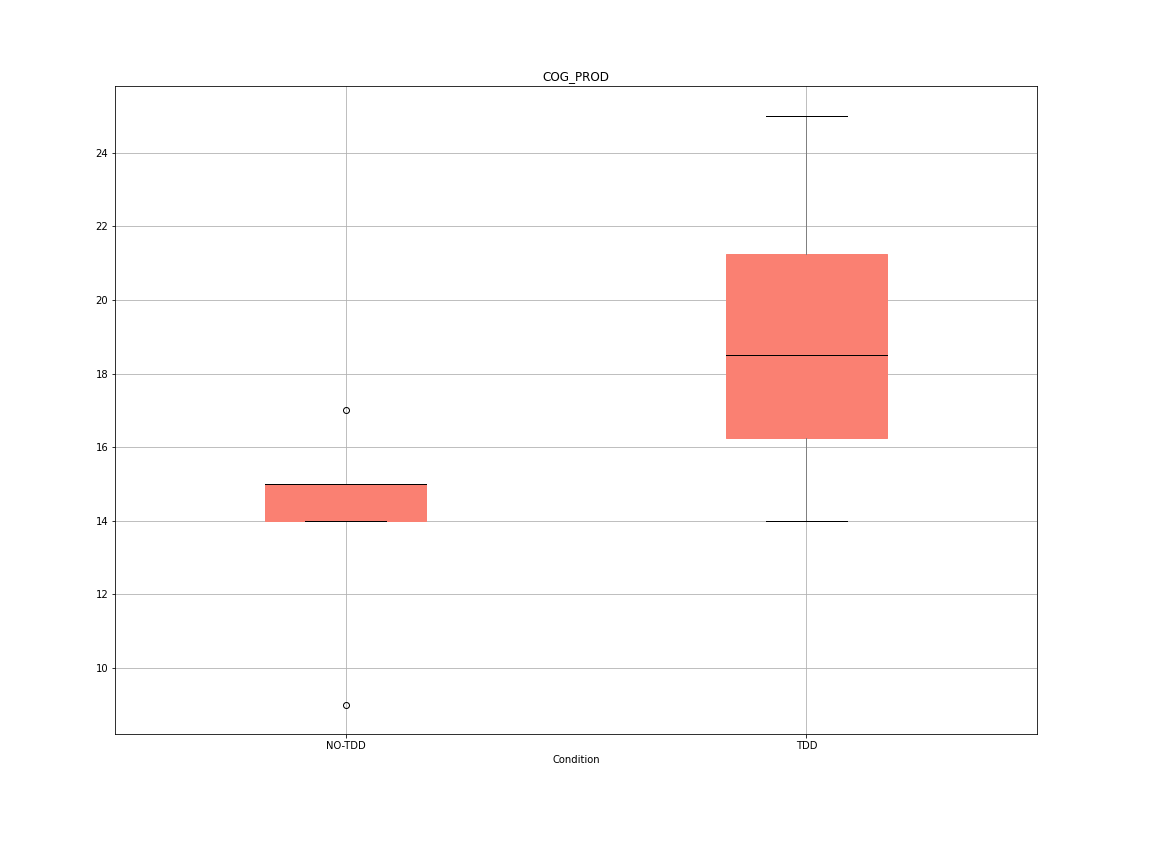
\includegraphics[width=\linewidth]{figures/box_plots/task1/COG.png}
        \caption{COG}
        \label{bp_task1_cog}
    \end{subfigure}\hfil
    \begin{subfigure}{0.33\textwidth}
        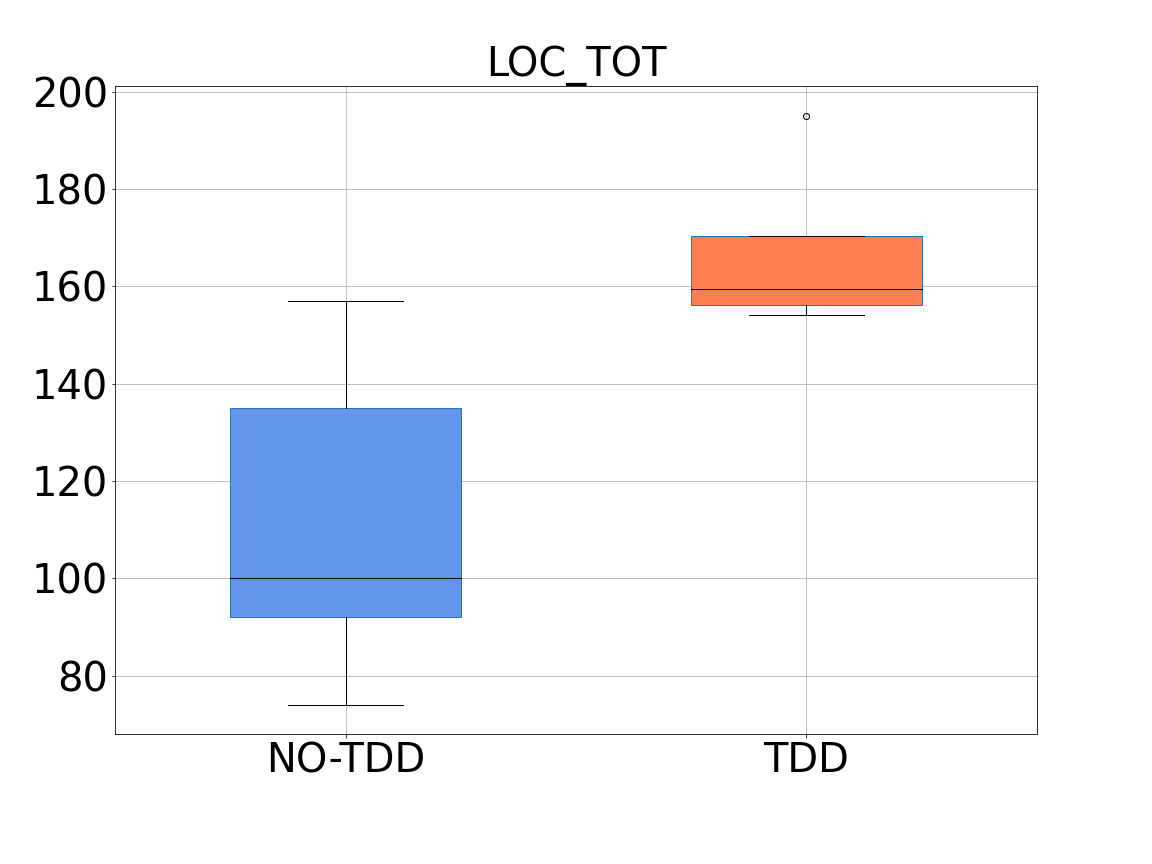
\includegraphics[width=\linewidth]{figures/box_plots/task1/LOC.png}
        \caption{LOC}
        \label{bp_task1_loc}
    \end{subfigure}
    \caption{Box plots for task 1, \textit{IntelligentOffice}.}
    \label{box_plots_task1}
\end{figure}



\begin{table}[!h]
    \begin{center} 
        \begin{tabular}{ |p{2cm}||p{1.6cm}|p{1.6cm}|p{1.6cm}|p{1.6cm}|p{1.6cm}|}
            \hline
                \multicolumn{6}{|c|}{Task 2 - TDD} \\
            \hline
                Metric & Min & Max & Mean & Median & Std\\
            \hline
                QLTY & 50 & 100 & 84.44 & 100 & 22.70 \\
                PROD & 8 & 100 & 38.6 & 21 & 37.35 \\
                TEST & 0 & 13 & 5.4 & 3 & 5.12 \\
                CYC & 9 & 19 & 12 & 10 & 4.06 \\
                COG & 2 & 40 & 12.8 & 4.0 & 15.91 \\
                LOC & 80 & 203 & 128 & 115 & 45.61 \\
            \hline
        \end{tabular}
        \caption{\label{tab_dv_t2_tdd}Dependent variables' statistics in task 2 for the \tdd group}
    \end{center}
\end{table}

\begin{table}[!h]
    \begin{center} 
        \begin{tabular}{ |p{2cm}||p{1.6cm}|p{1.6cm}|p{1.6cm}|p{1.6cm}|p{1.6cm}|}
            \hline
                \multicolumn{6}{|c|}{Task 2 - NO-TDD} \\
            \hline
                Metric & Min & Max & Mean & Median & Std\\
            \hline
                QLTY & 74 & 94.43 & 83.07 & 81.94 & 10.17 \\
                PROD & 52 & 73 & 60.5 & 58.5 & 10.24 \\
                TEST & 5 & 12 & 9 & 9.5 & 2.94 \\
                CYC & 16 & 36 & 23.5 & 21 & 9 \\
                COG & 11 & 49 & 29 & 28 & 15.57 \\
                LOC & 178 & 260 & 207.5 & 196 & 37.11 \\
            \hline
        \end{tabular}
        \caption{\label{tab_dv_t2_notdd}Dependent variables' statistics in task 2 for the \notdd group}
    \end{center}
\end{table}

\begin{figure}[htbp]
    \centering
    \begin{subfigure}{0.33\textwidth}
        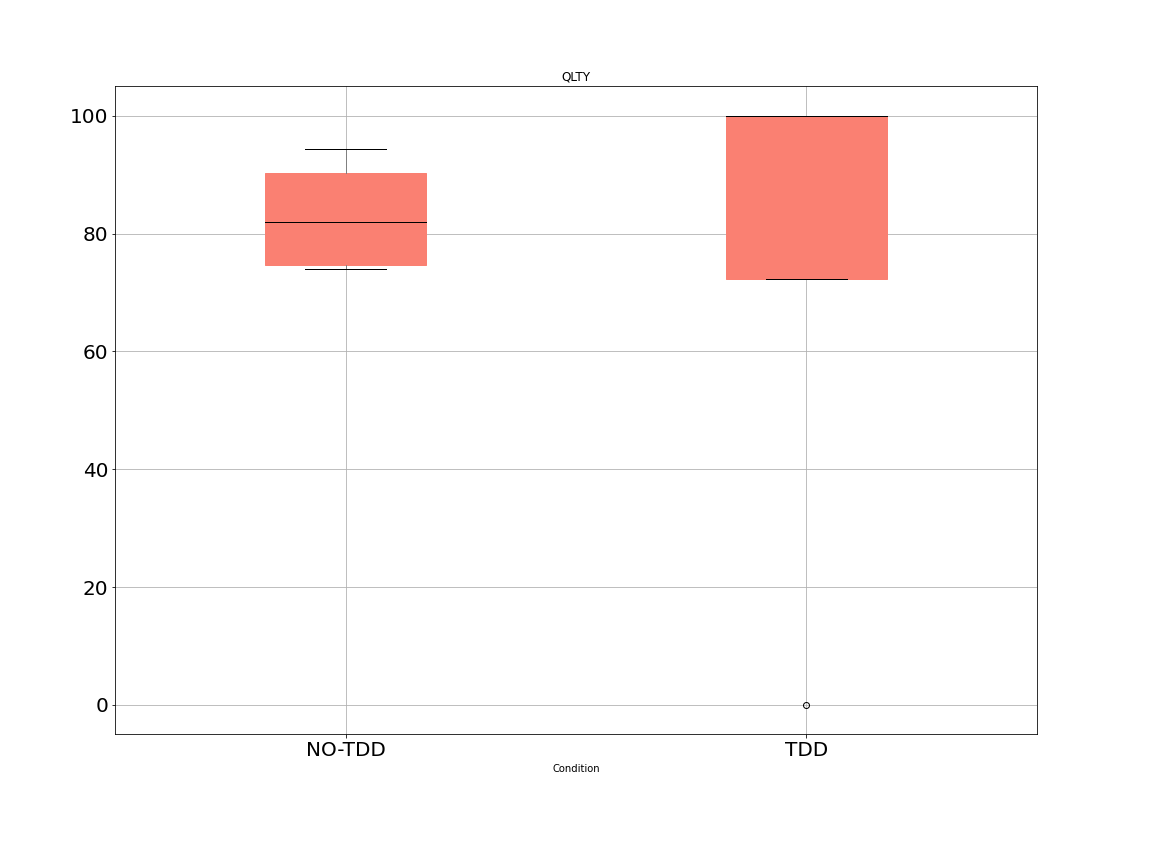
\includegraphics[width=\linewidth]{figures/box_plots/task2/QLTY.png}
        \caption{QLTY}
        \label{bp_task2_qlty}
    \end{subfigure}\hfil
        \begin{subfigure}{0.33\textwidth}
        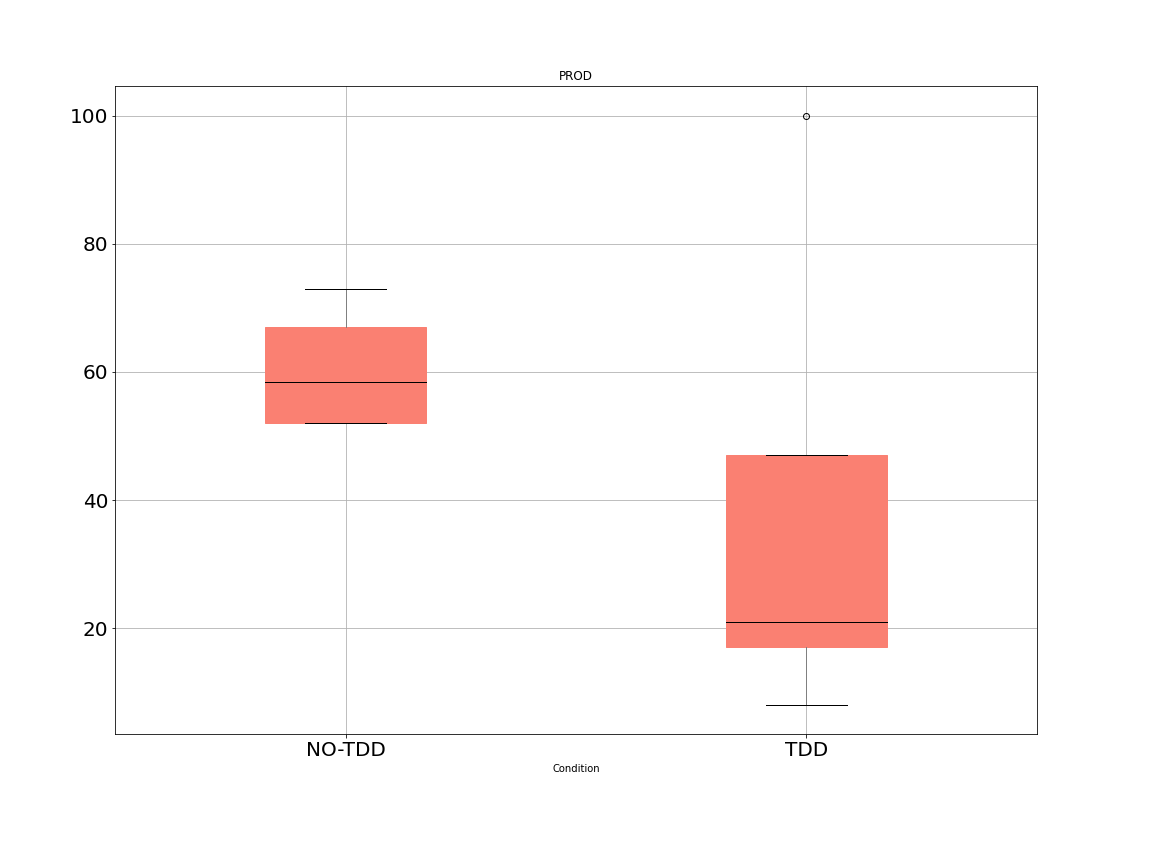
\includegraphics[width=\linewidth]{figures/box_plots/task2/PROD.png}
        \caption{PROD}
        \label{bp_task2_prod}
    \end{subfigure}\hfil
    \begin{subfigure}{0.33\textwidth}
        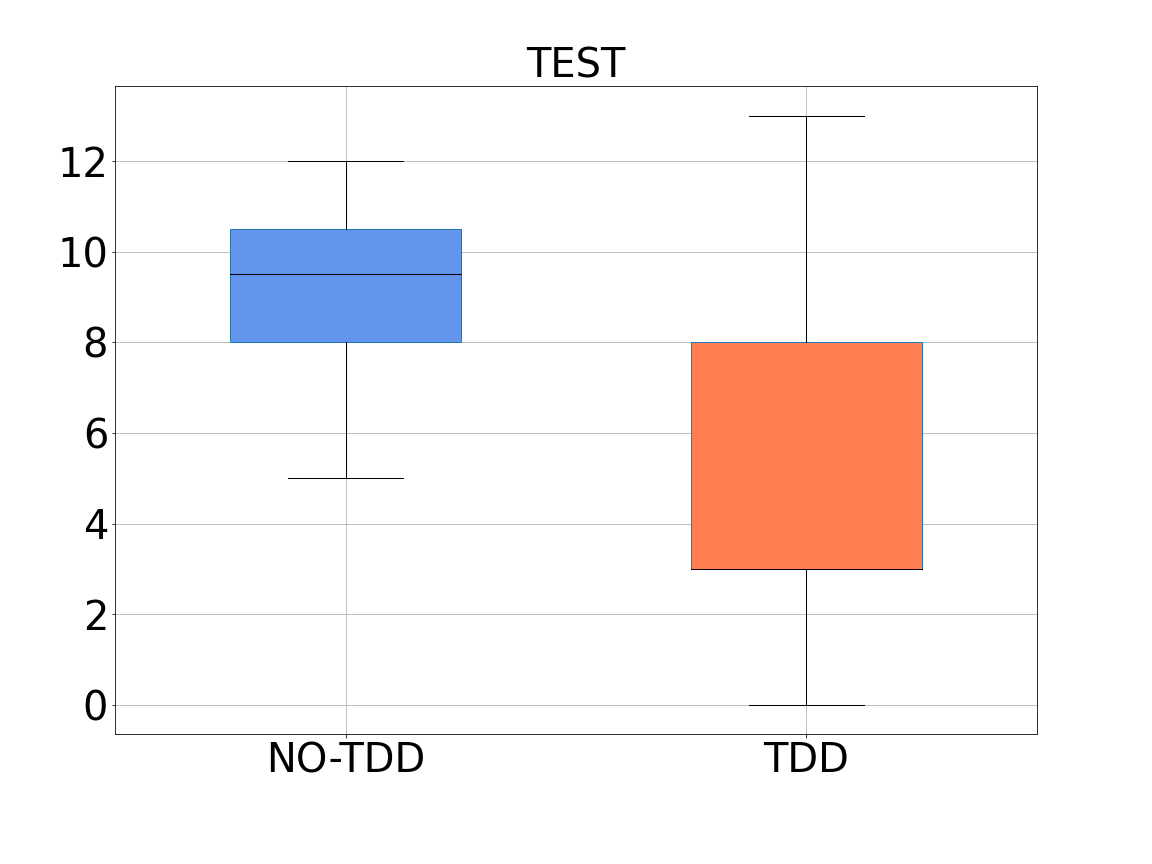
\includegraphics[width=\linewidth]{figures/box_plots/task2/TEST.png}
        \caption{TEST}
        \label{bp_task2_test}
    \end{subfigure}

    \medskip
    \begin{subfigure}{0.33\textwidth}
        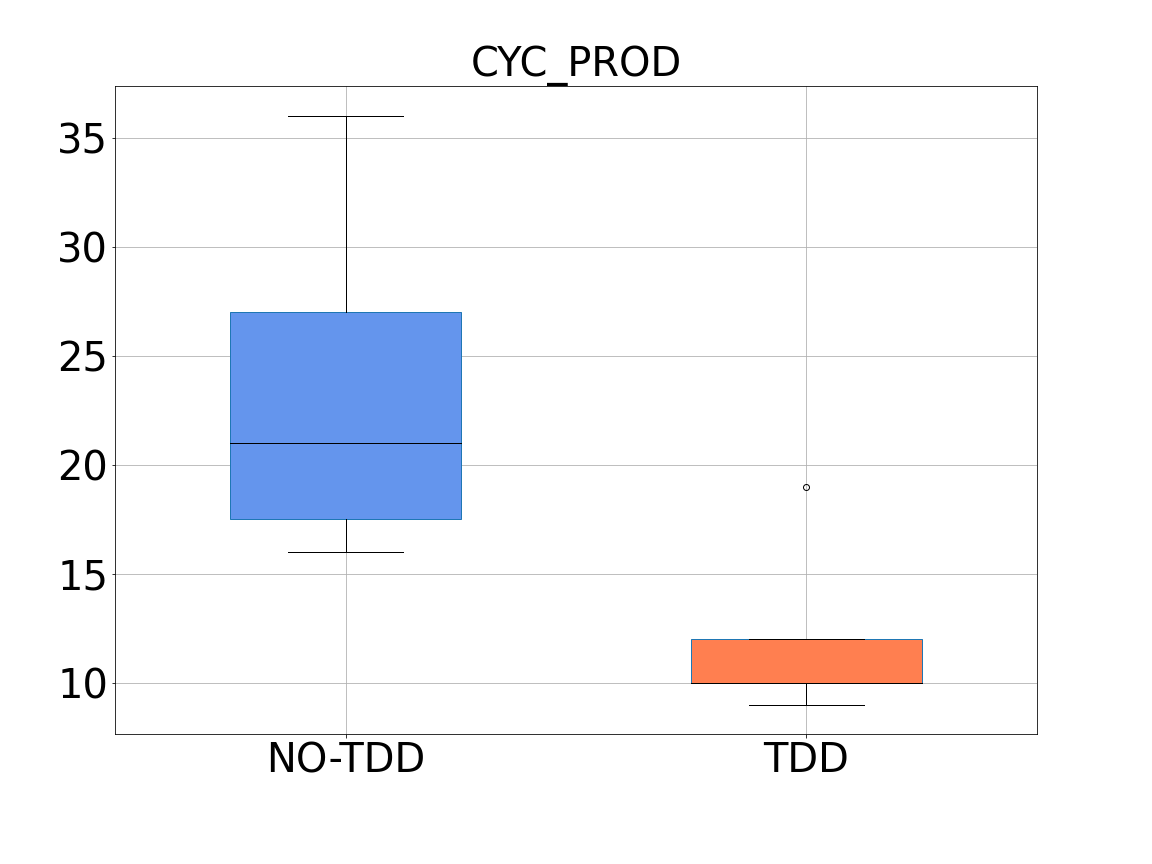
\includegraphics[width=\linewidth]{figures/box_plots/task2/CYC.png}
        \caption{CYC}
        \label{bp_task2_cyc}
    \end{subfigure}\hfil
    \begin{subfigure}{0.33\textwidth}
        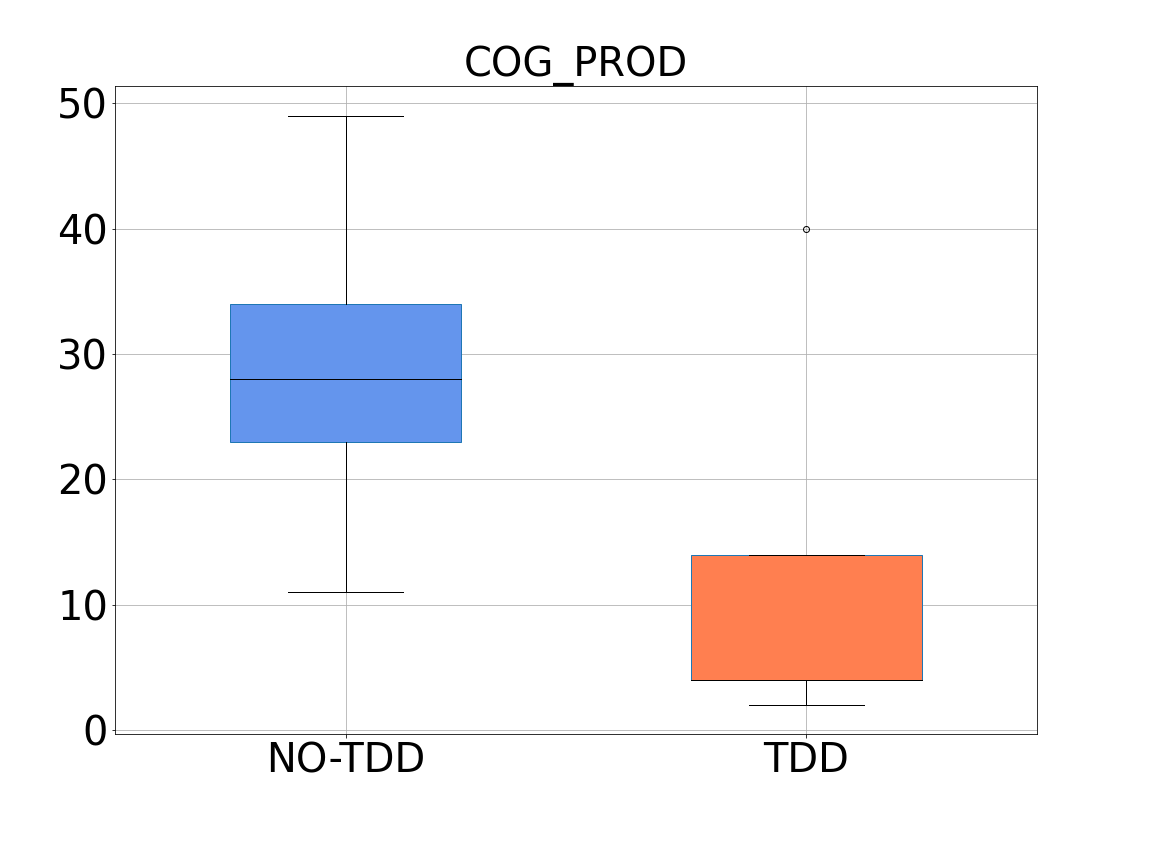
\includegraphics[width=\linewidth]{figures/box_plots/task2/COG.png}
        \caption{COG}
        \label{bp_task2_cog}
    \end{subfigure}\hfil
    \begin{subfigure}{0.33\textwidth}
        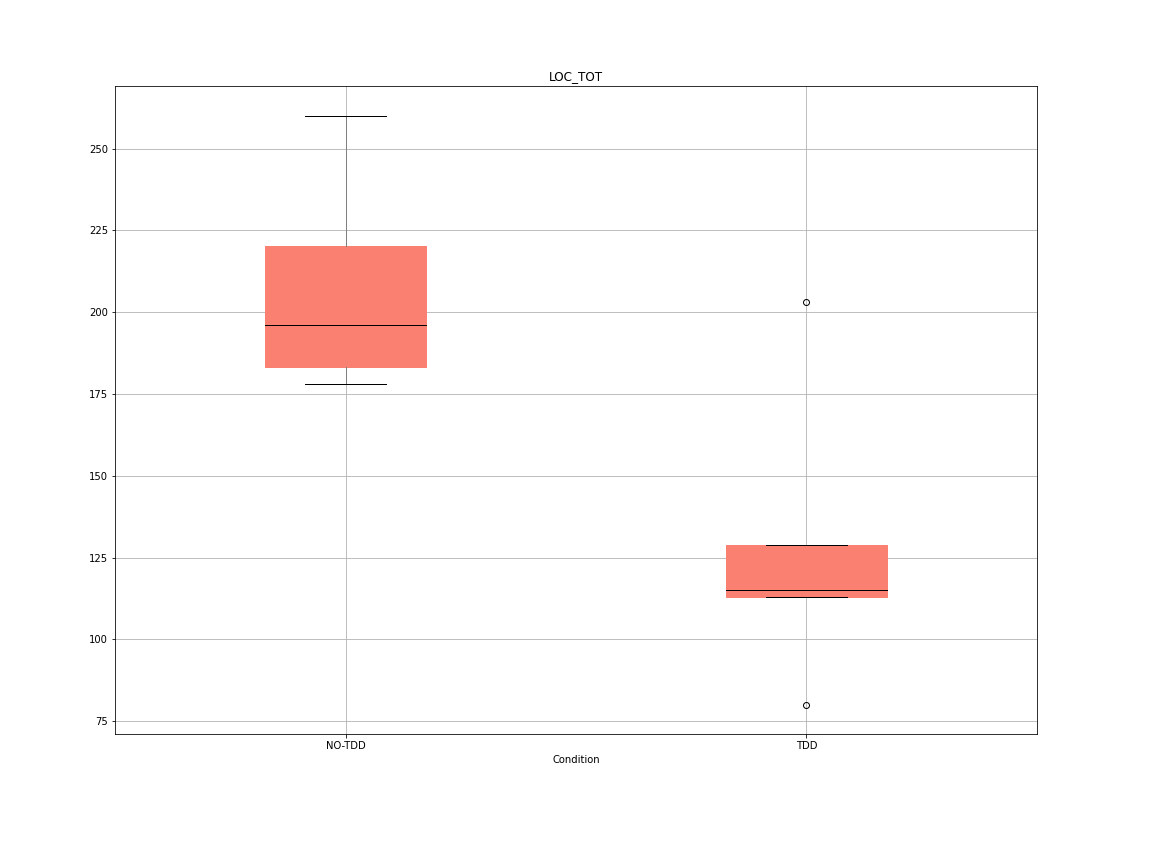
\includegraphics[width=\linewidth]{figures/box_plots/task2/LOC.png}
        \caption{LOC}
        \label{bp_task2_loc}
    \end{subfigure}
    \caption{Box plots for task 2, \textit{CleaningRobot}.}
    \label{box_plots_task2}
\end{figure}



\begin{table}[!h]
    \begin{center} 
        \begin{tabular}{ |p{2cm}||p{1.6cm}|p{1.6cm}|p{1.6cm}|p{1.6cm}|p{1.6cm}|}
            \hline
                \multicolumn{6}{|c|}{Task 1 \& 2 - TDD} \\
            \hline
                Metric & Min & Max & Mean & Median & Std\\
            \hline
                QLTY & 50 & 100 & 82.97 & 82 & 17.43 \\
                PROD & 8 & 100 & 58.33 & 72 & 35.76 \\
                TEST & 0 & 13 & 7.22 & 8 & 4.26 \\
                CYC & 9 & 28 & 17.66 & 19 & 7.51 \\
                COG & 2 & 40 & 15.55 & 14 & 12.06 \\
                LOC & 80 & 203 & 145.33 & 154 & 39.97 \\
            \hline
        \end{tabular}
        \caption{\label{tab_dv_t1_2_tdd}Dependent variables' statistics in tasks 1 and 2 for the \tdd group}
    \end{center}
\end{table}

\begin{table}[!h]
    \begin{center} 
        \begin{tabular}{ |p{2cm}||p{1.6cm}|p{1.6cm}|p{1.6cm}|p{1.6cm}|p{1.6cm}|}
            \hline
                \multicolumn{6}{|c|}{Task 1 \& 2 - NO-TDD} \\
            \hline
                Metric & Min & Max & Mean & Median & Std\\
            \hline
                QLTY & 65.55 & 94.43 & 78.78 & 78.77 & 9.11 \\
                PROD & 52 & 84 & 69.11 & 73 & 13.22 \\
                TEST & 0 & 12 & 6.11 & 7.0 & 5.08 \\
                CYC & 12 & 36 & 19.11 & 16 & 7.07 \\
                COG & 9 & 49 & 20.66 & 15 & 12.56 \\
                LOC & 74 & 260 & 154.22 & 157 & 60.32 \\
            \hline
        \end{tabular}
        \caption{\label{tab_dv_t1_2_notdd}Dependent variables' statistics in tasks 1 and 2 for the \notdd group}
    \end{center}
\end{table}

\begin{figure}[htbp]
    \centering
    \begin{subfigure}{0.33\textwidth}
        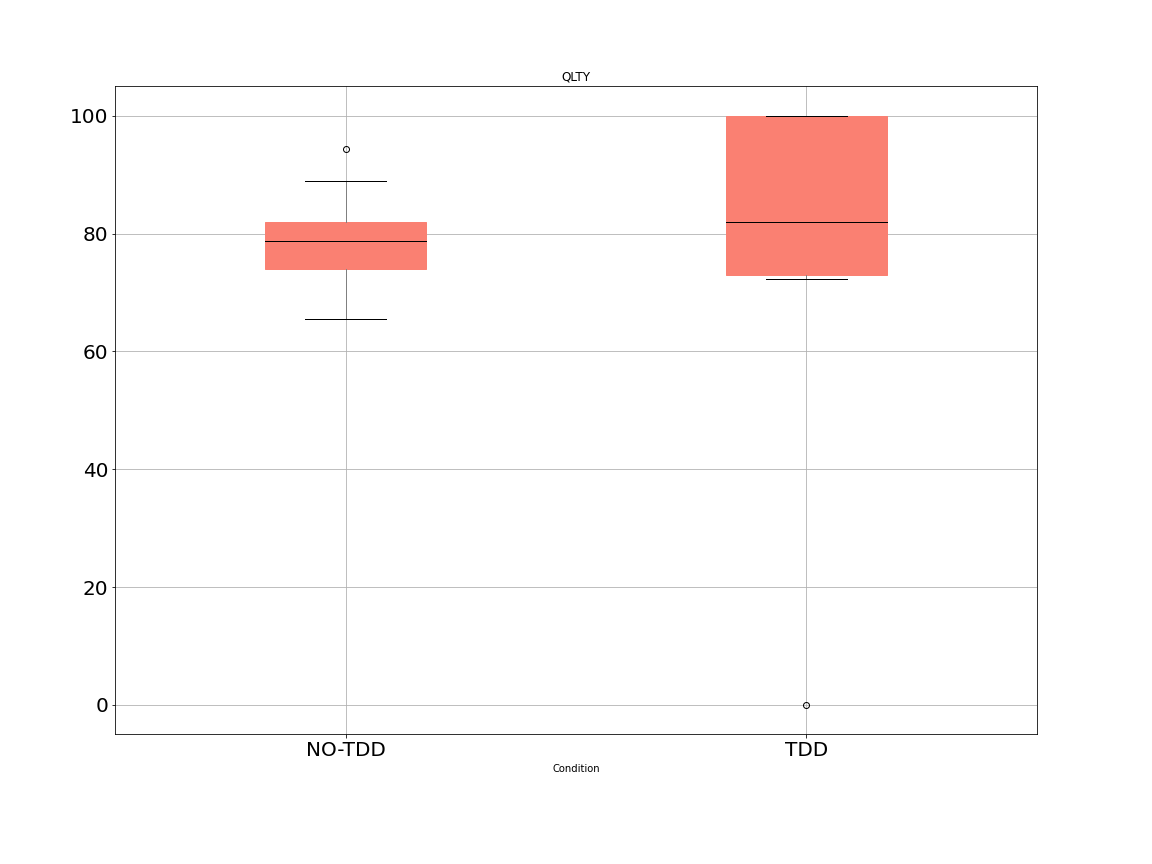
\includegraphics[width=\linewidth]{figures/box_plots/task1_2/QLTY.png}
        \caption{QLTY}
        \label{bp_task1_2_qlty}
    \end{subfigure}\hfil
        \begin{subfigure}{0.33\textwidth}
        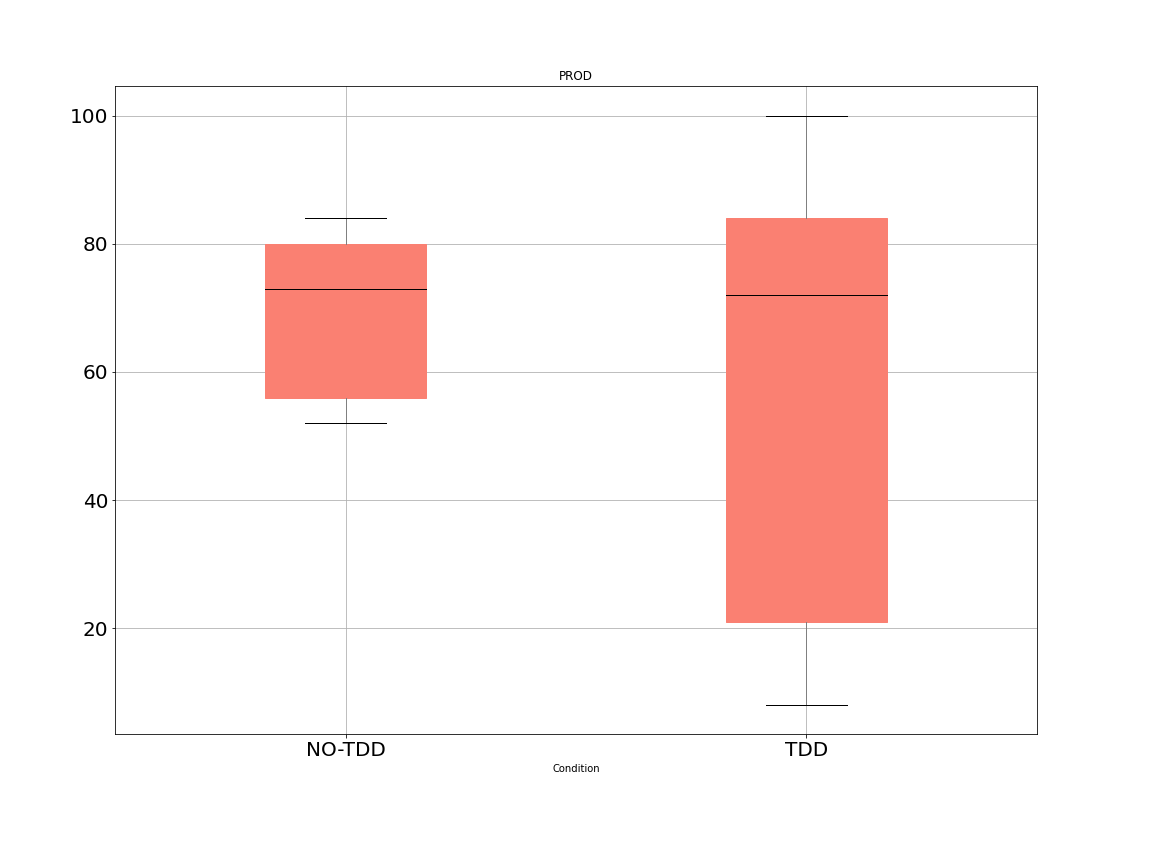
\includegraphics[width=\linewidth]{figures/box_plots/task1_2/PROD.png}
        \caption{PROD}
        \label{bp_task1_2_prod}
    \end{subfigure}\hfil
    \begin{subfigure}{0.33\textwidth}
        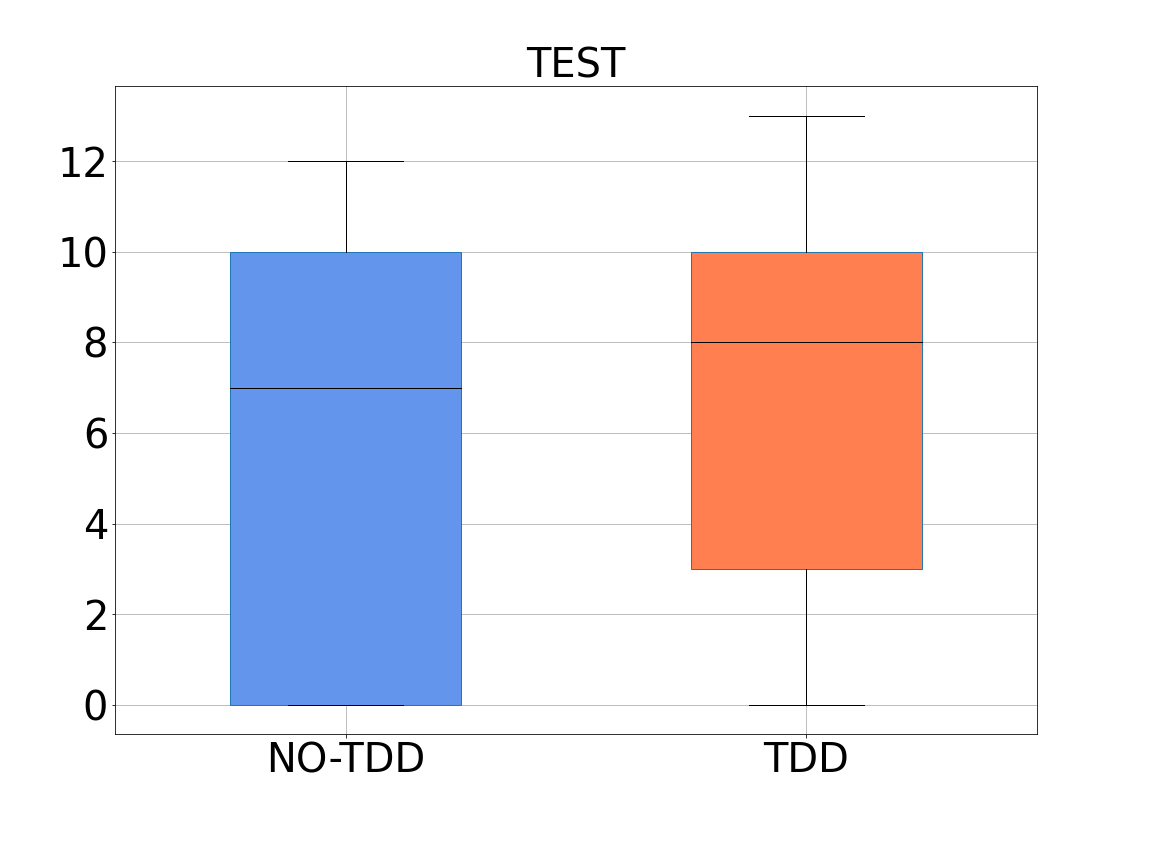
\includegraphics[width=\linewidth]{figures/box_plots/task1_2/TEST.png}
        \caption{TEST}
        \label{bp_task1_2_test}
    \end{subfigure}

    \medskip
    \begin{subfigure}{0.33\textwidth}
        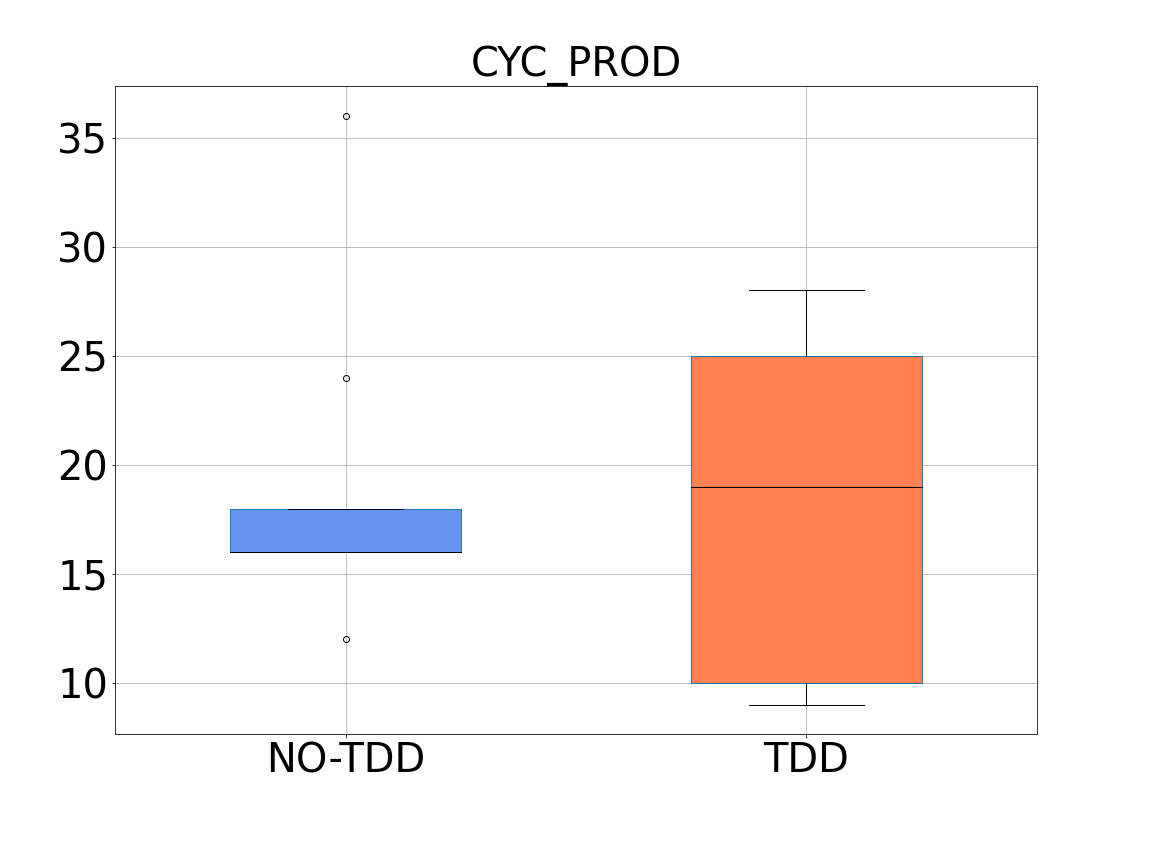
\includegraphics[width=\linewidth]{figures/box_plots/task1_2/CYC.png}
        \caption{CYC}
        \label{bp_task1_2_cyc}
    \end{subfigure}\hfil
    \begin{subfigure}{0.33\textwidth}
        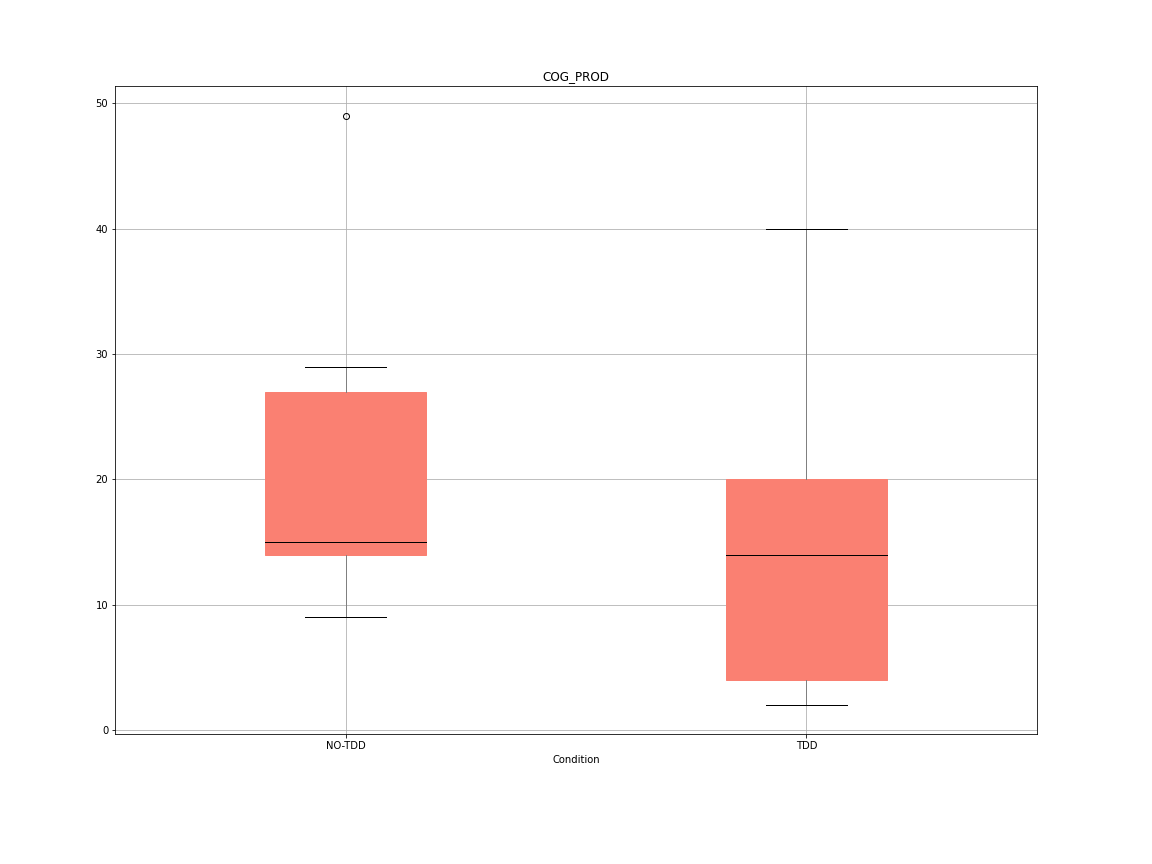
\includegraphics[width=\linewidth]{figures/box_plots/task1_2/COG.png}
        \caption{COG}
        \label{bp_task1_2_cog}
    \end{subfigure}\hfil
    \begin{subfigure}{0.33\textwidth}
        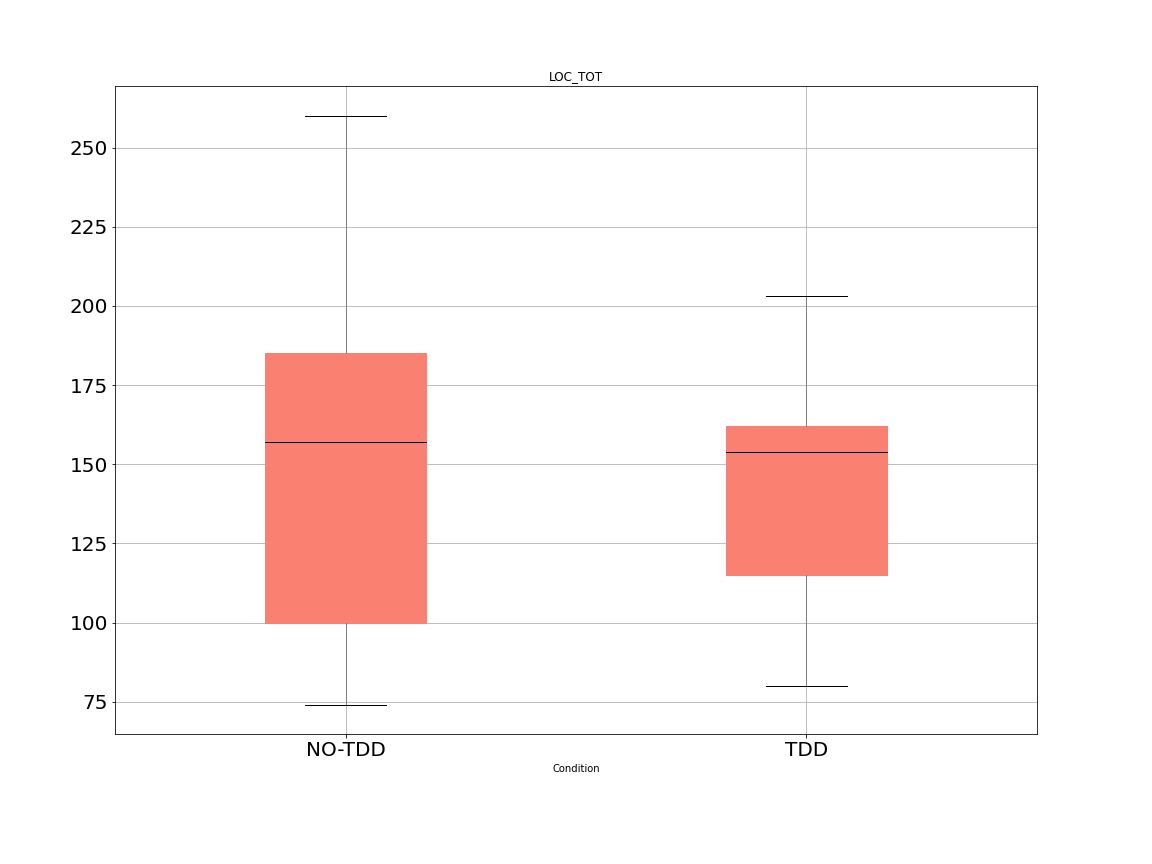
\includegraphics[width=\linewidth]{figures/box_plots/task1_2/LOC.png}
        \caption{LOC}
        \label{bp_task1_2_loc}
    \end{subfigure}
    \caption{Aggregated box plots for tasks 1 and 2.}
    \label{box_plots_task1_2}
\end{figure}



\begin{table}[!h]
    \begin{center} 
        \begin{tabular}{ |p{2cm}||p{1.6cm}|p{1.6cm}|p{1.6cm}|p{1.6cm}|p{1.6cm}|}
            \hline
                \multicolumn{6}{|c|}{Task 3 - TDD} \\
            \hline
                Metric & Min & Max & Mean & Median & Std\\
            \hline
                QLTY & 85 & 100 & 95 & 100 & 7.07 \\
                PROD & 83.33 & 100 & 93.33 & 100 & 9.13 \\
                TEST & 7 & 18 & 11.6 & 12 & 4.15 \\
                CYC & 15 & 30 & 22.6 & 20 & 6.58 \\
                COG & 18 & 34 & 25.8 & 25 & 7.08 \\
                LOC & 150 & 232 & 187 & 175 & 36.15 \\
            \hline
        \end{tabular}
        \caption{\label{tab_dv_t3_tdd}Dependent variables' statistics in task 3 for the \tdd group}
    \end{center}
\end{table}

\begin{table}[!h]
    \begin{center} 
        \begin{tabular}{ |p{2cm}||p{1.6cm}|p{1.6cm}|p{1.6cm}|p{1.6cm}|p{1.6cm}|}
            \hline
                \multicolumn{6}{|c|}{Task 3 - NO-TDD} \\
            \hline
                Metric & Min & Max & Mean & Median & Std\\
            \hline
                QLTY & 80 & 100 & 86.25 & 82.5 & 9.46 \\
                PROD & 75 & 100 & 83.33 & 79.16 & 11.78 \\
                TEST & 0 & 11 & 4.5 & 3.5 & 5.44 \\
                CYC & 16 & 23 & 19.5 & 19.5 & 2.88 \\
                COG & 19 & 25 & 21 & 20 & 2.70 \\
                LOC & 93 & 164 & 125.5 & 122.5 & 36.82 \\
            \hline
        \end{tabular}
        \caption{\label{tab_dv_t3_notdd}Dependent variables' statistics in task 3 for the \notdd group}
    \end{center}
\end{table}

\begin{figure}[htbp]
    \centering
    \begin{subfigure}{0.33\textwidth}
        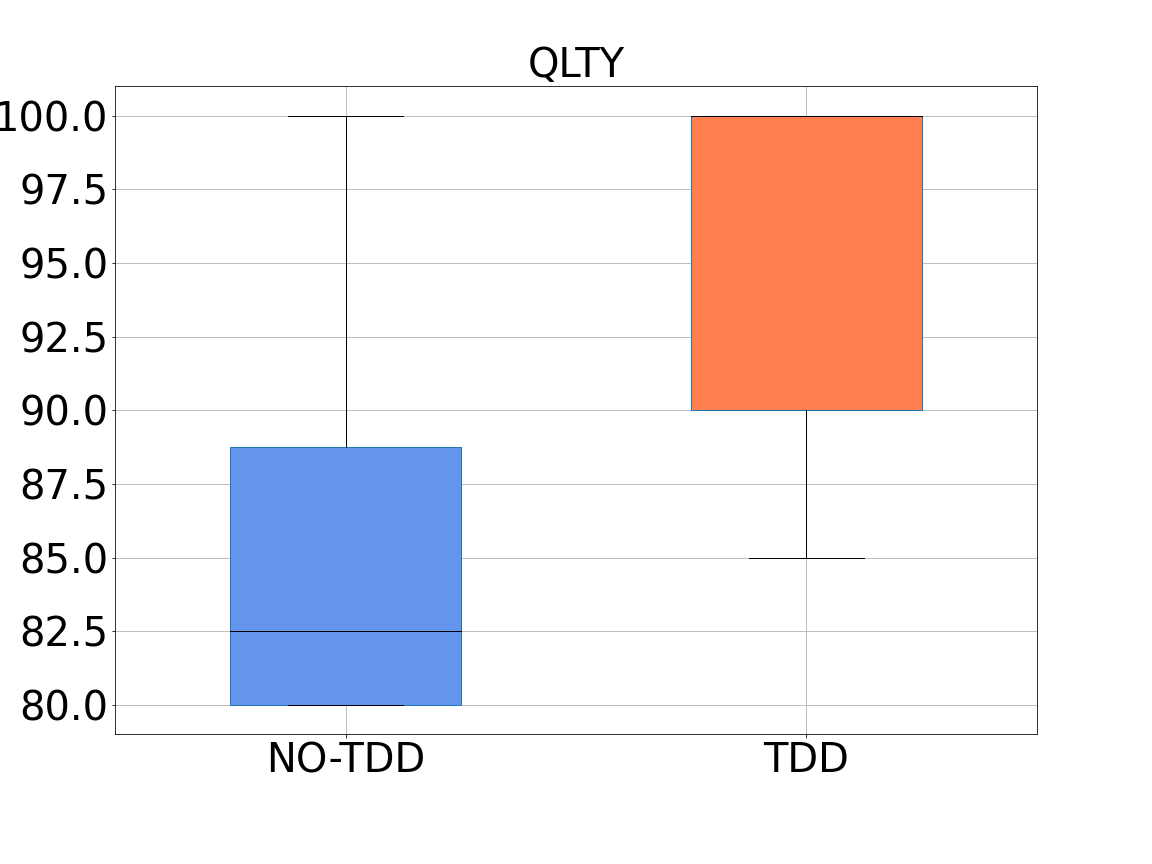
\includegraphics[width=\linewidth]{figures/box_plots/task3/QLTY.png}
        \caption{QLTY}
        \label{bp_task3_qlty}
    \end{subfigure}\hfil
        \begin{subfigure}{0.33\textwidth}
        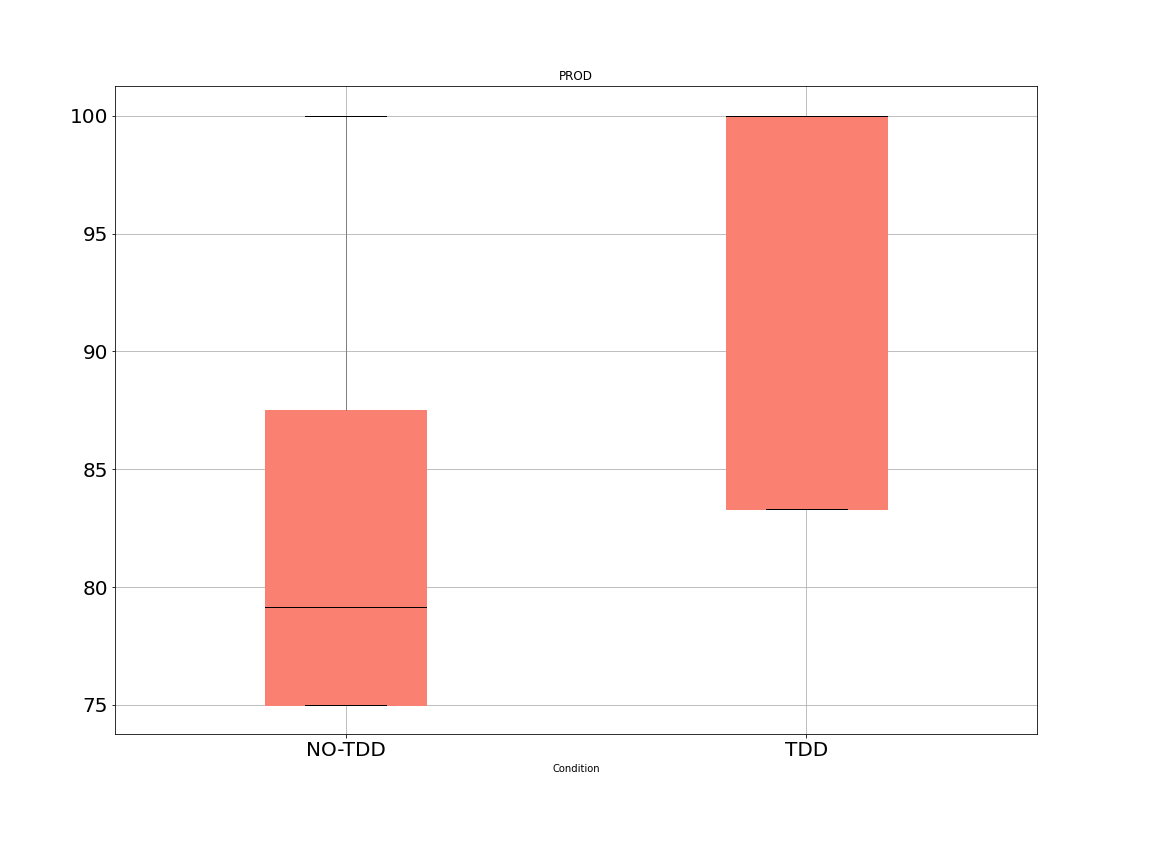
\includegraphics[width=\linewidth]{figures/box_plots/task3/PROD.png}
        \caption{PROD}
        \label{bp_task3_prod}
    \end{subfigure}\hfil
    \begin{subfigure}{0.33\textwidth}
        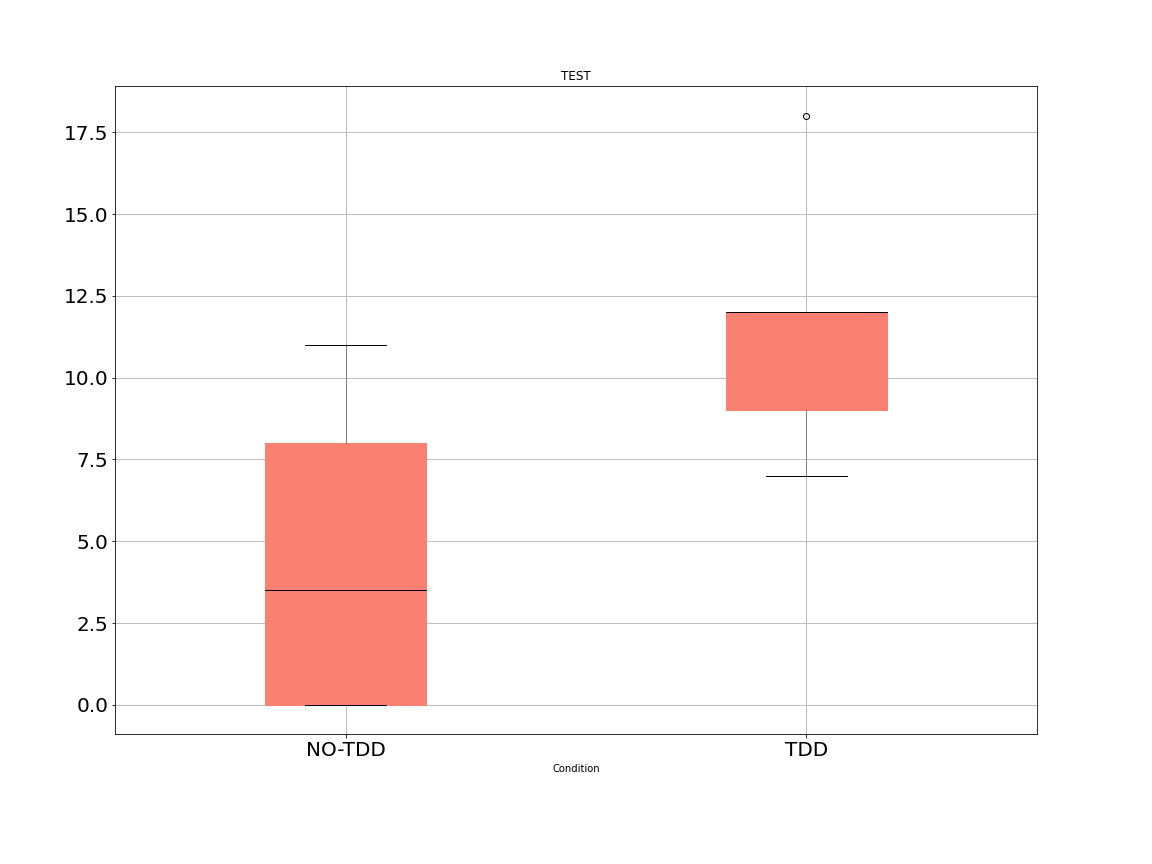
\includegraphics[width=\linewidth]{figures/box_plots/task3/TEST.png}
        \caption{TEST}
        \label{bp_task3_test}
    \end{subfigure}

    \medskip
    \begin{subfigure}{0.33\textwidth}
        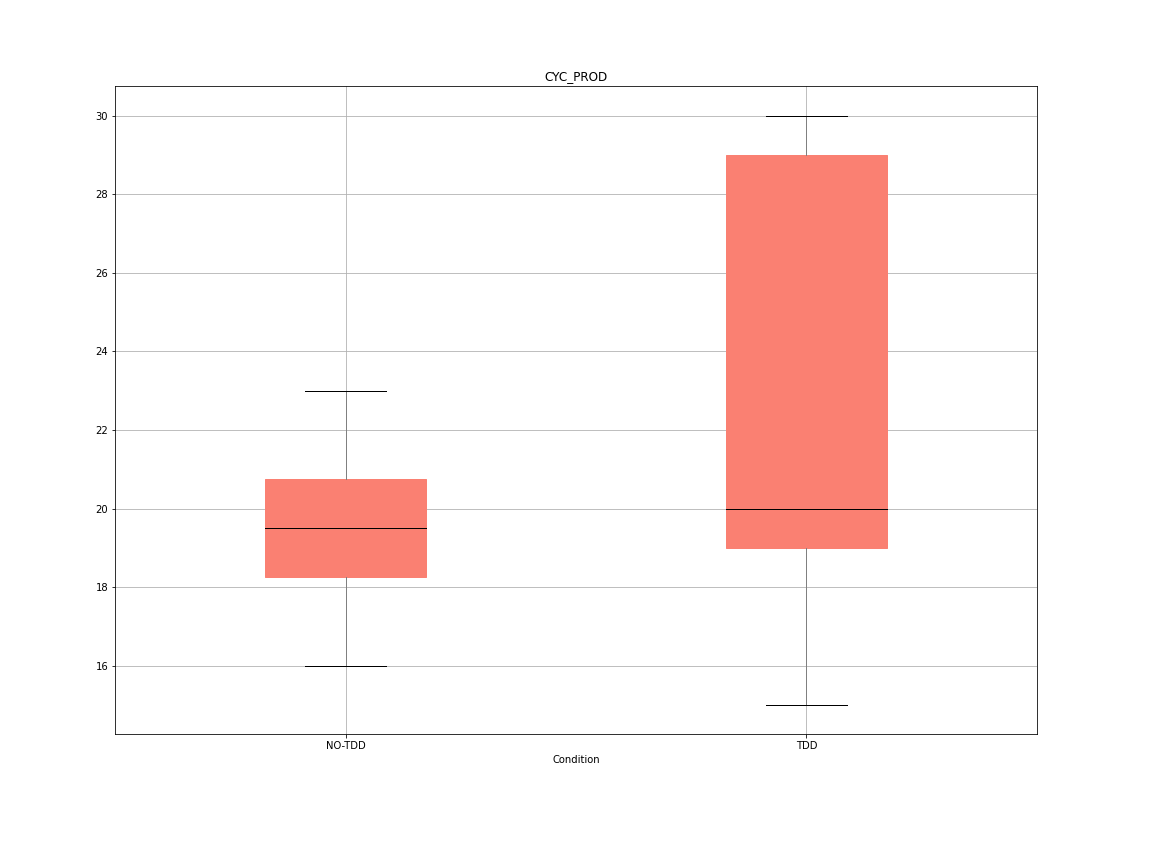
\includegraphics[width=\linewidth]{figures/box_plots/task3/CYC.png}
        \caption{CYC}
        \label{bp_task3_cyc}
    \end{subfigure}\hfil
    \begin{subfigure}{0.33\textwidth}
        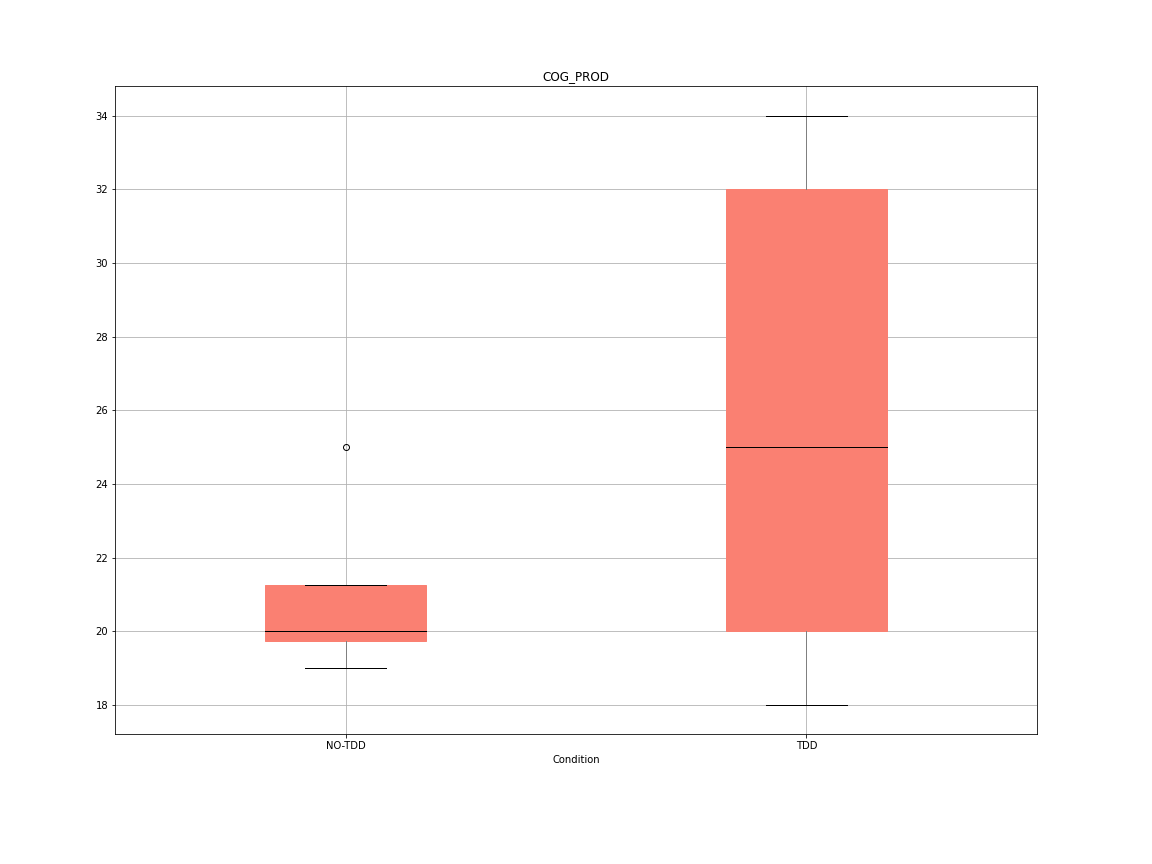
\includegraphics[width=\linewidth]{figures/box_plots/task3/COG.png}
        \caption{COG}
        \label{bp_task3_cog}
    \end{subfigure}\hfil
    \begin{subfigure}{0.33\textwidth}
        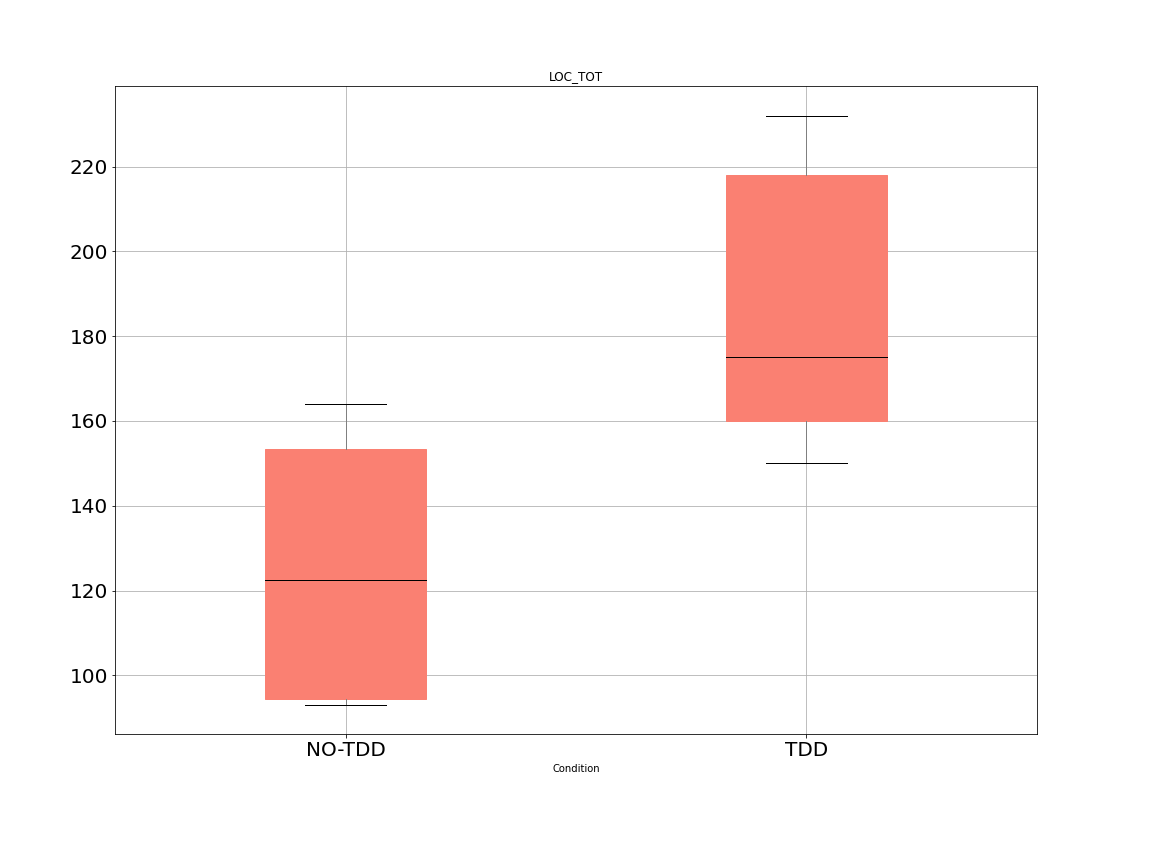
\includegraphics[width=\linewidth]{figures/box_plots/task3/LOC.png}
        \caption{LOC}
        \label{bp_task3_loc}
    \end{subfigure}
    \caption{Box plots for task 3, \textit{SmartHome}.}
    \label{box_plots_task3}
\end{figure}

\subsection{Meta-analysis}
The following figures display the results of the aggregate analysis on the variables of the baseline and replication studies through means of forest plot charts, one per variable. These plots report the Standard Mean Difference (SMD)and the corresponding 95\% Confidence Intervals (CIs), two statistics to assess between-study heterogeneity: the p-value from the Q-test and the $I^2$ statistic [12]  


was chosen as the effect measure, as suggested 

\begin{figure}[htbp]
    \centering
    \begin{subfigure}{0.5\textwidth}
        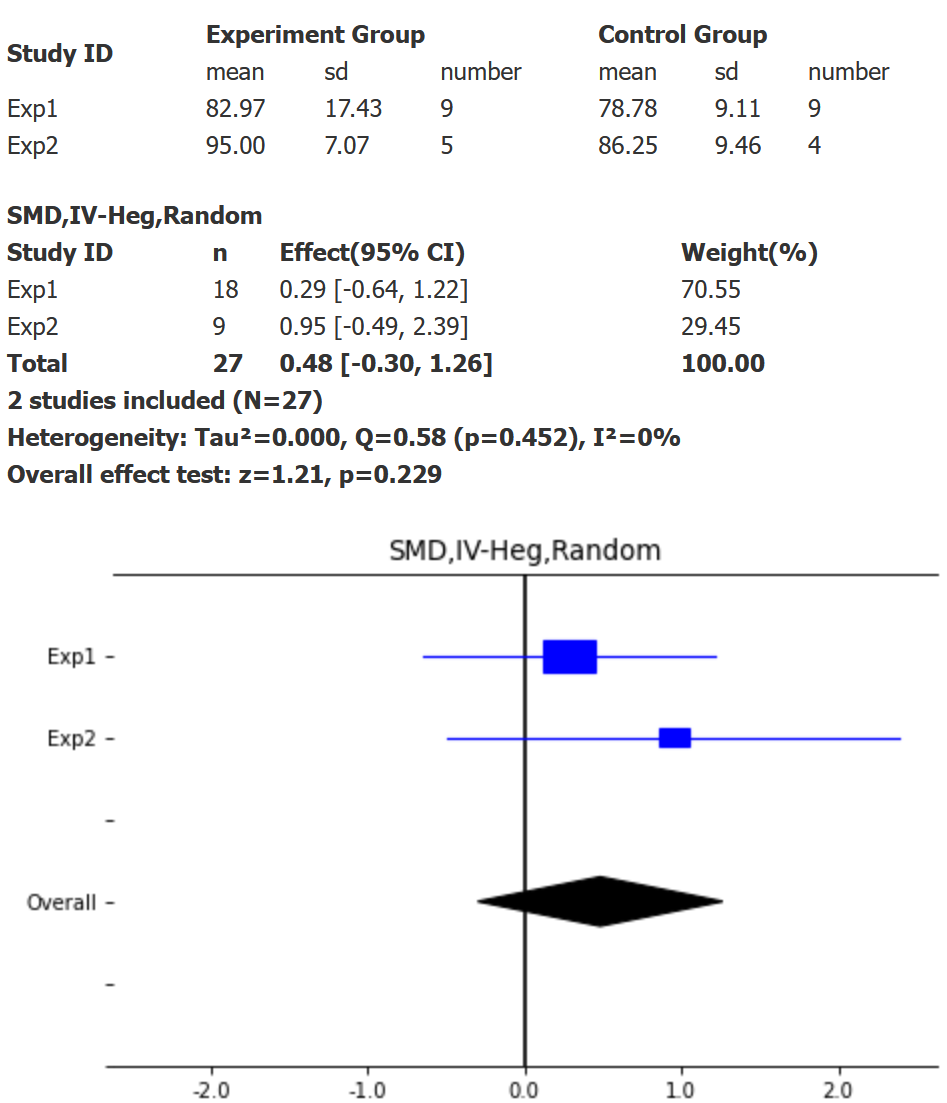
\includegraphics[width=\linewidth]{figures/forest_plots/QLTY.png}
        \caption{QLTY}
        \label{fp1}
    \end{subfigure}\hfil
    \begin{subfigure}{0.5\textwidth}
        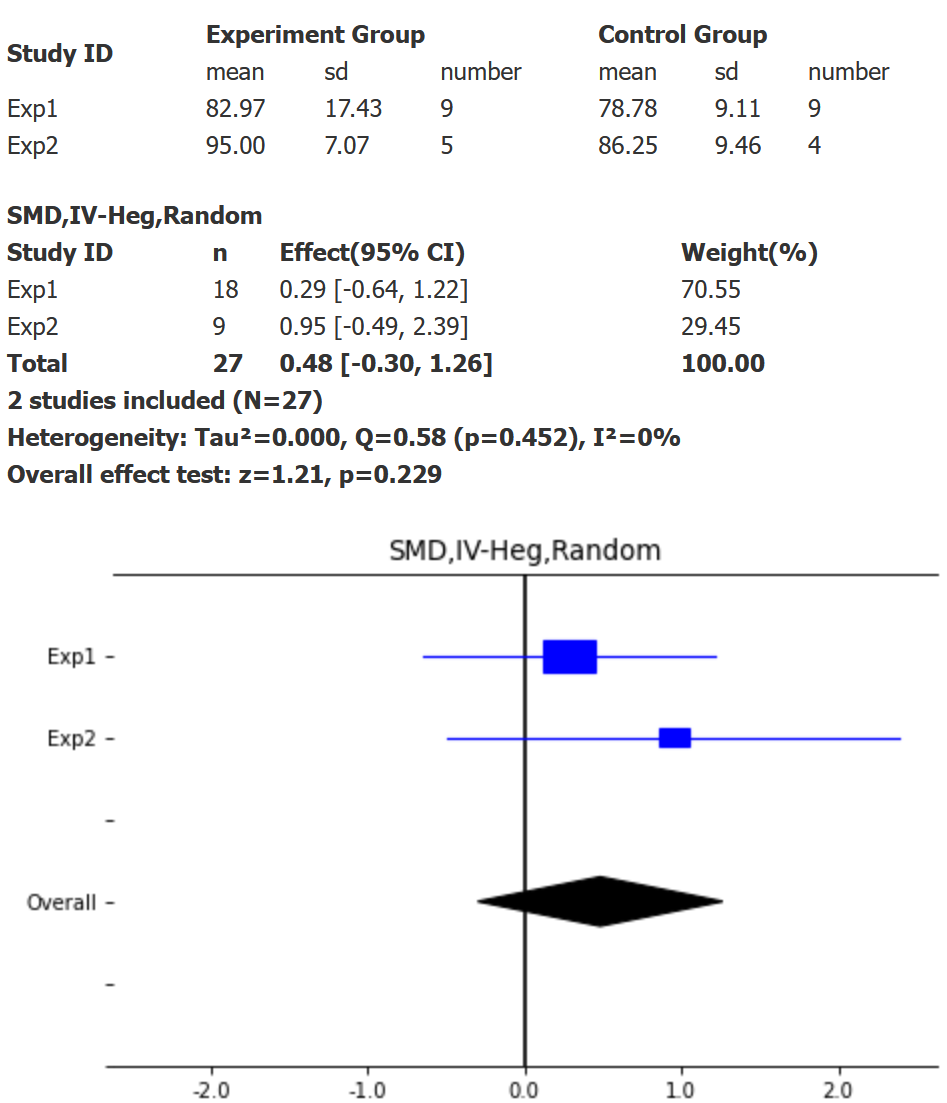
\includegraphics[width=\linewidth]{figures/forest_plots/QLTY.png}
        \caption{PROD}
        \label{fp2}
    \end{subfigure}

    \medskip

    \begin{subfigure}{0.5\textwidth}
        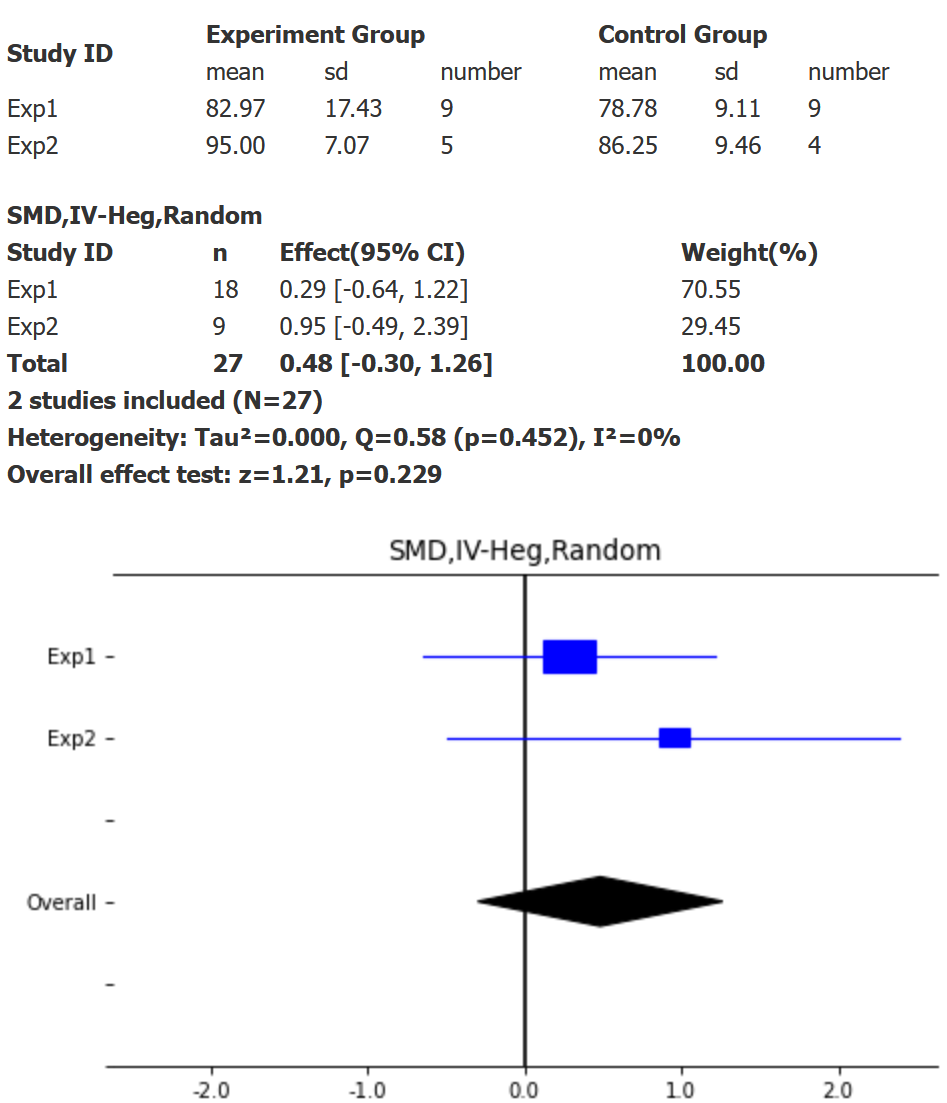
\includegraphics[width=\linewidth]{figures/forest_plots/QLTY.png}
        \caption{TEST}
        \label{fp3}
    \end{subfigure}\hfil
    \begin{subfigure}{0.5\textwidth}
        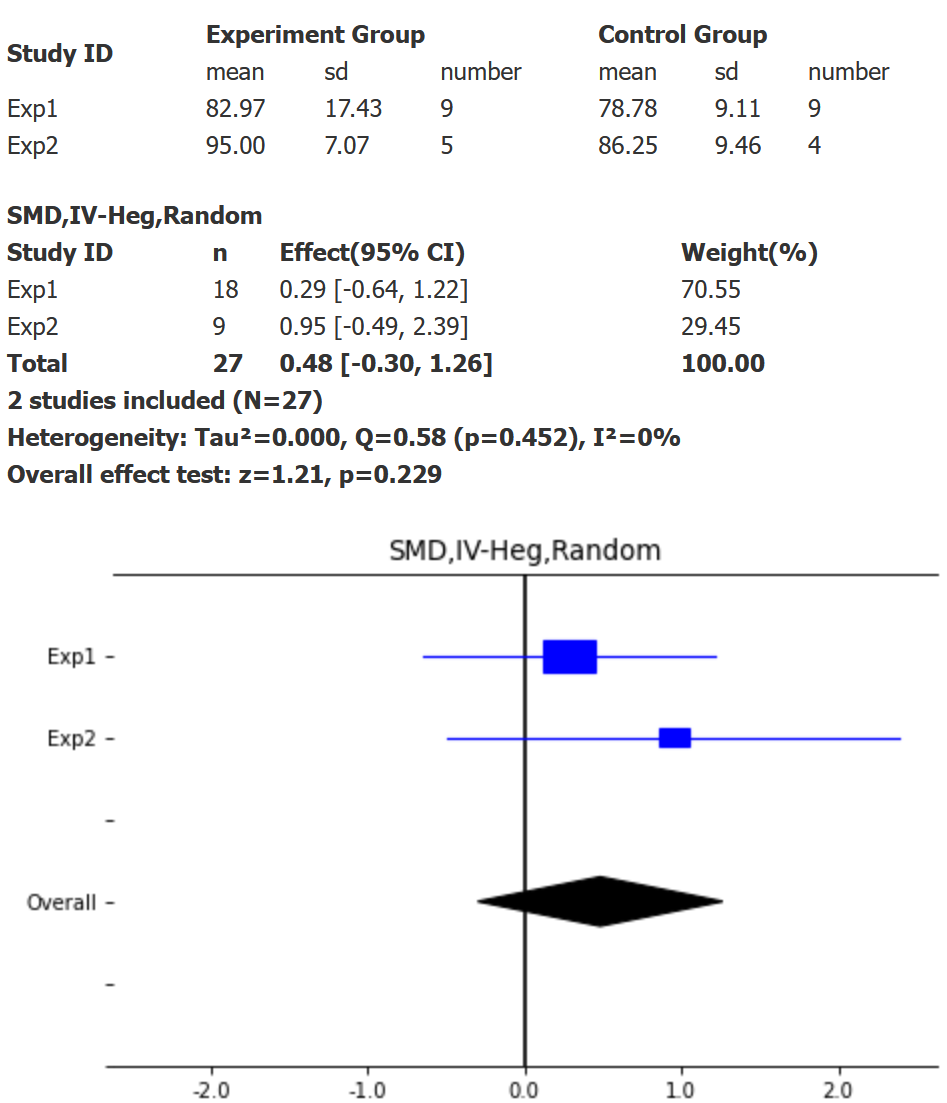
\includegraphics[width=\linewidth]{figures/forest_plots/QLTY.png}
        \caption{CYC}
        \label{fp4}
    \end{subfigure}

    \medskip

    \begin{subfigure}{0.5\textwidth}
        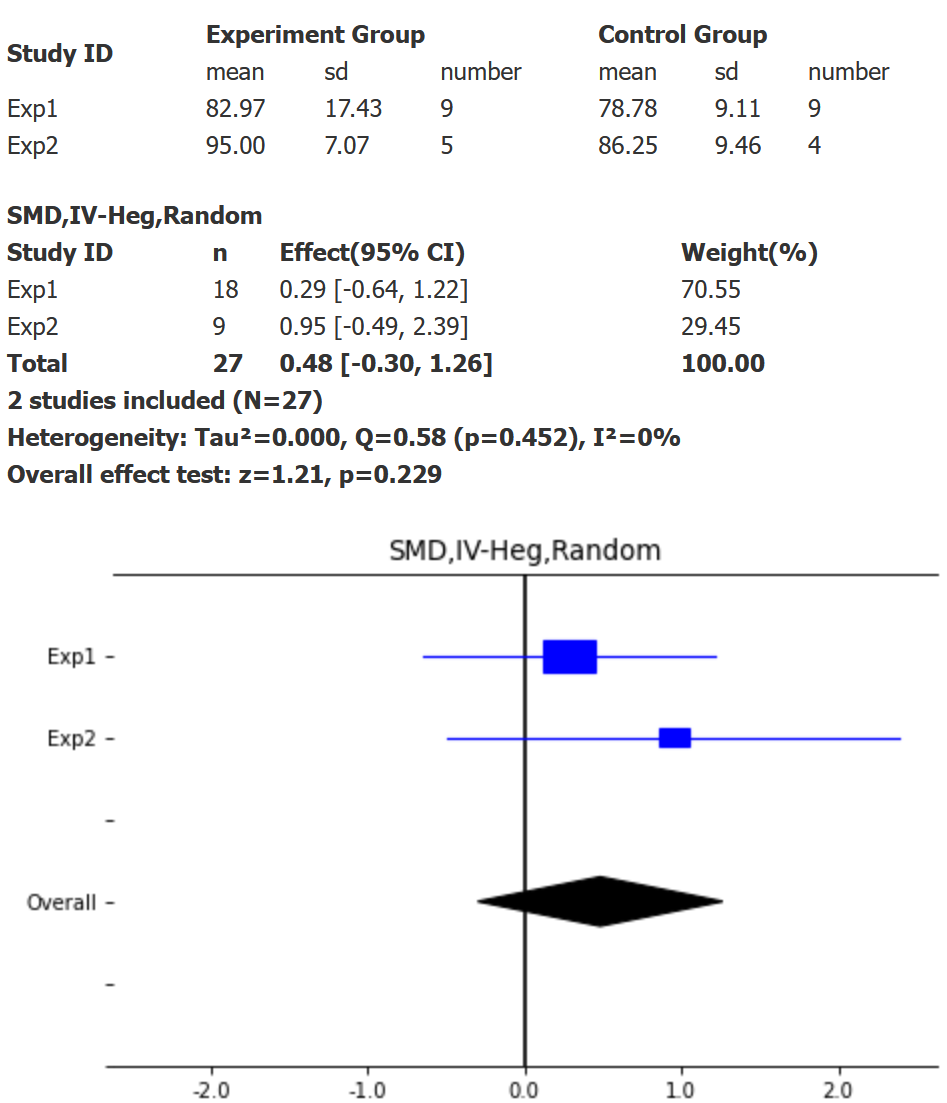
\includegraphics[width=\linewidth]{figures/forest_plots/QLTY.png}
        \caption{COG}
        \label{fp5}
    \end{subfigure}\hfil
    \begin{subfigure}{0.5\textwidth}
        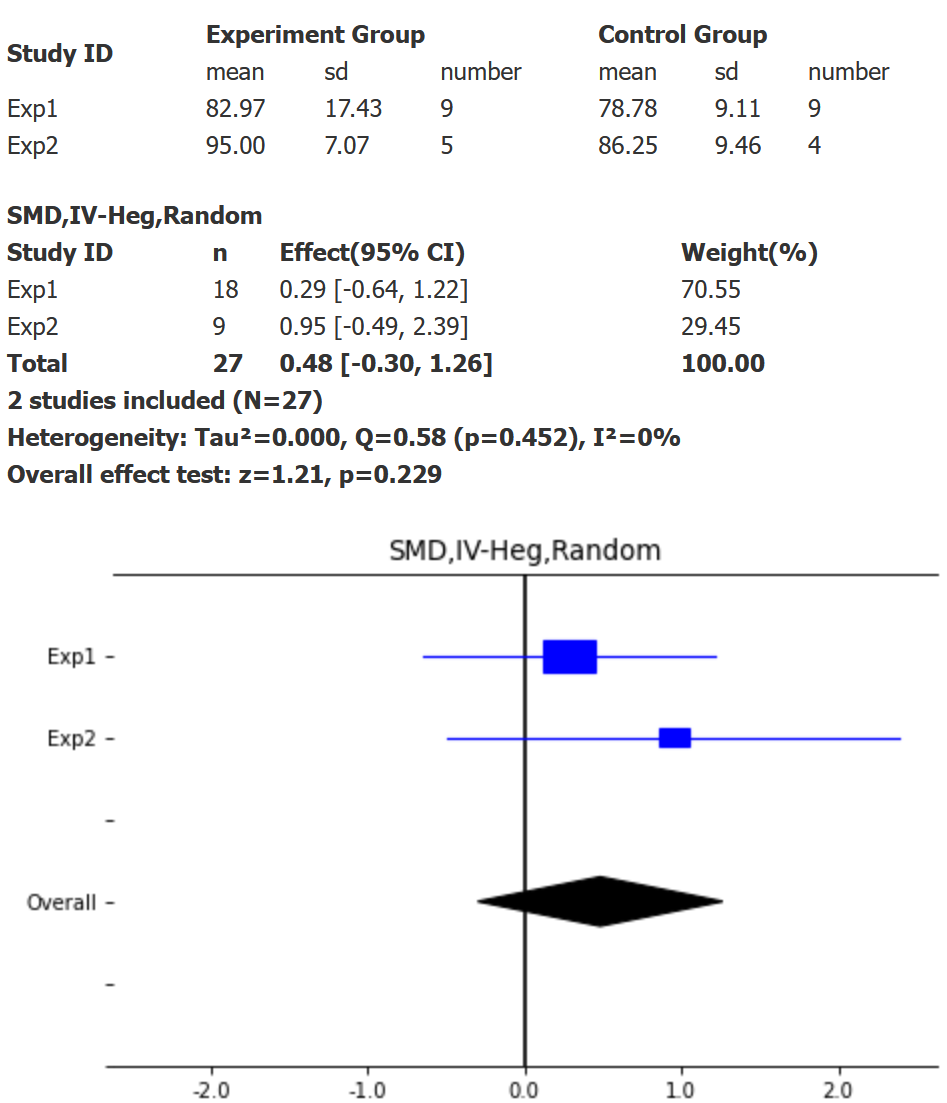
\includegraphics[width=\linewidth]{figures/forest_plots/QLTY.png}
        \caption{LOC}
        \label{fp6}
    \end{subfigure}
    \caption{Box plots for task 1, \textit{IntelligentOffice}}
    \label{fpx}
\end{figure}

\begin{figure}[H]
    \centering
    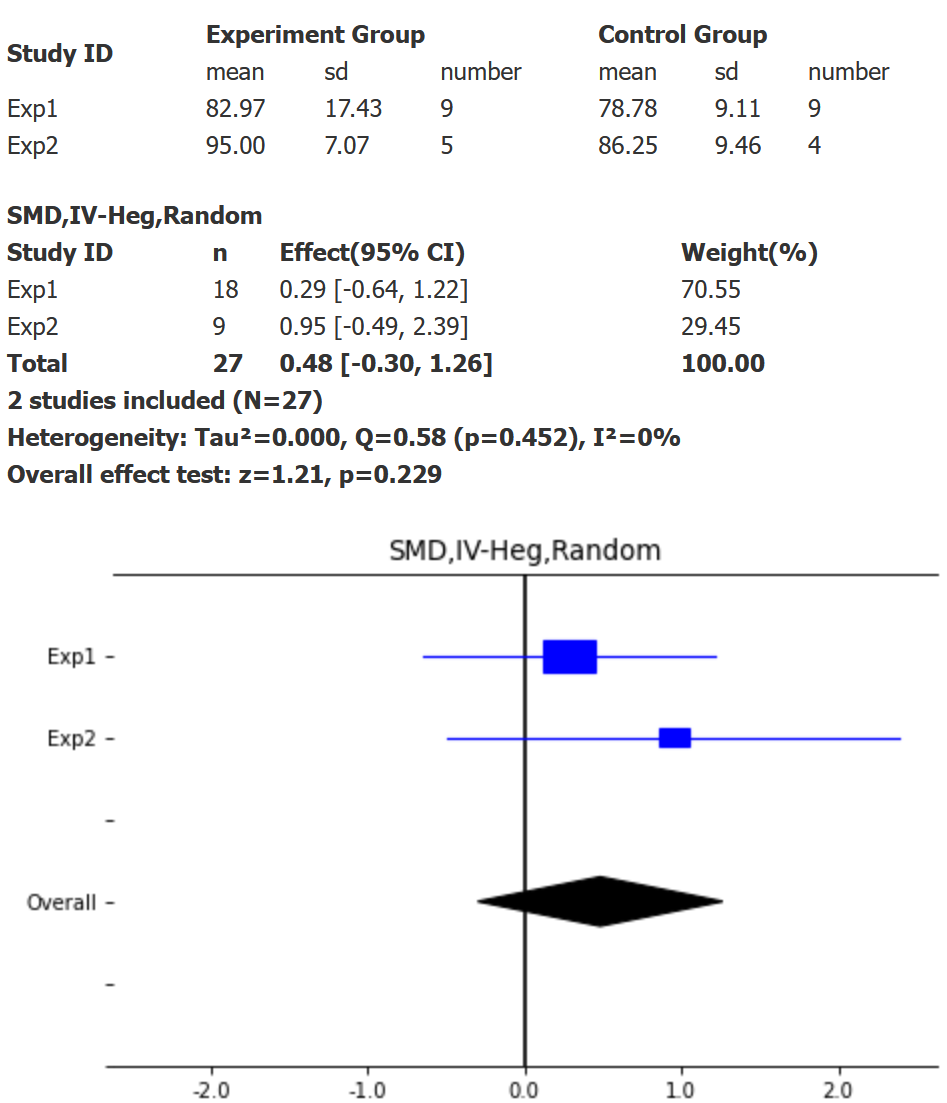
\includegraphics[width=\linewidth]{figures/forest_plots/QLTY.png}
    \caption{Forest plot chart for the QLTY dependent variable}
    \label{forest_plot}
\end{figure}



\subsection{Post-questionnaire Analysis}
Fig \ref{bar_charts} summarizes the answers provided by the participants in the post-experiment questionnaires, comparing the responses by the employed condition (\tdd or \notdd).
Regarding user story comprehensibility, in the first experimental task, \textit{IntelligentOffice}, the majority of participants have a similar agreement on the matter, with percentages of agreement of 88\% (\tdd) and 80\% (\notdd). As for the second task, \textit{CleaningRobot}, there is a more substantial difference, with only 40\% of the \tdd group having a positive perception of the user stories' comprehensibility, compared to the 87\% of the \notdd group.

A similar trend can be noted for the second question, regarding the general task feasibility; here, in the first experimental task, the participants somewhat agree, with 50\% of the \tdd group and 40\% of the \notdd group feeling neutral about the difficulty of the task. In the second task, the answers are quite mixed, with 40\% of the participants in the \tdd finding the task at hand very difficult to understand, and the other 60\% equally split between finding the task hard, feeling neutral about it or considering it very easy.  On the other hand, all of the participants in the \notdd group agreed on feeling neutral about their ease in developing it.

Finally, question three was focused on the difficulty of the participants in applying their reference condition (\ie \tdd or \notdd): for task 1, the \tdd group did not have a strong opinion on applying this technique, with 76\% feeling neutral about it, and the other 24\% finding the application of \tdd easy but not too easy; The \notdd group had also the majority of opinions feeling neutral about their approach (60\%), however this time 20\% of the participants felt very good about applying \notdd; this is probably due to their seniority with the approach.


\begin{figure}[htbp]
    \begin{subfigure}{\textwidth}
        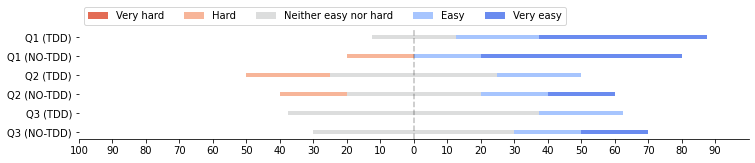
\includegraphics[width=\textwidth]{figures/bar_charts/task1.png}
        \caption{First experimental task, \textit{IntelligentOffice}}
    \end{subfigure}
    
    \bigskip
    
    \begin{subfigure}{\textwidth}
        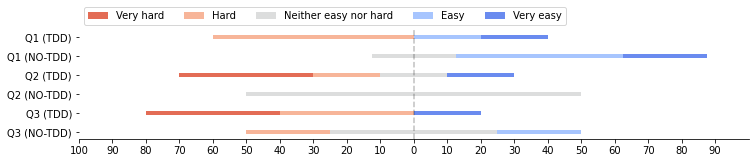
\includegraphics[width=\textwidth]{figures/bar_charts/task2.png}
        \caption{Second experimental task, \textit{CleaningRobot}}
    \end{subfigure}
    
    \caption{Diverging stacked bar charts for the post-questionnaires}
    \label{bar_charts}
\end{figure}

As for the open-ended question, we performed thematic analysis in order to identify a base template on which to parse the answers provided by the participants in the post-questionnaires after the two tasks of the baseline study.
The themes that we identified are:
\begin{enumerate}
    \item Feelings on the development task.
    \item Feelings on \tdd to accomplish the task.
    \item Feelings on \notdd to accomplish the task.
    \item Personal comparison thoughts between \tdd and \notdd.
\end{enumerate}

Most of the participants found the first development task not particularly challenging, with 6 out of 9 participants expressing a positive feeling about it; 2 out of the remaining 3 found some challenges and would have liked a bit more time, while the last participant did not answer. 
For task 2, 2 out of 9 students had no issues with the task, while 6 found the task to be harder than the previous one: out of the latter, 3 reported struggling with implementing some user stories, while 3 simply stated that the task was more challenging, without voicing their struggles with it.
Employing \tdd to approach the tasks was still not fully clear at the end of the first two tasks. For task 1, 2 participants expressed how getting into the \tdd mindset for a new task was not easy, while another student found this practice very useful and expressed their good feelings for having learned it. 
In the second task, which was considered overall hardware, 3 out of five participants in the \tdd group expressed having trouble with it.
As for the chosen \notdd approach, in the first task 3 out 5 participants dealing with this testing approach still wrote test cases after the production code, while the other 2 chose not to; for the second task, all 4 participants in the \notdd group tested their implementation.
At the end of the second task, 4 participants expressed their preference with \tdd, while 3 were still more comfortable with \notdd. Finally, the last participant expressed how in their opinion the best approach to use depended on the requirement quality  for development task.

Thematic analysis was also used to extract patterns from the final individual participant interview; the template identified the following main topics: 
\begin{enumerate}
    \item Thoughts on the replication experiment.
    \item Refactoring with \tdd.
    \item \notdd testing approach.
    \item Applying \tdd for \ess development.
    \item Prior participant testing experience.
    \item ThoughtS on the overall experience with the studies, from the lectures and homeworks to the last development task.
\end{enumerate}

For the first point, 5 out of 9 participants found the task straight forward and had no issues with its development, while the other 4 found it balanced, with some user stories requiring more thought before being implemented. Furthermore, 3 participants were already familiar with some of the sensors and actuators used for the task, either from previous university courses, or from personal experience.
For this last task, 5 out of 9 participants were assigned the \tdd version, while the other 4 had to develop the \es using \notdd; out of the 5 that used \tdd, 4 of them performed some refactoring, while 1 did not. As for the \notdd group, half still wrote tests after implementing the user stories, while the other half did not.

To the questions "What can be done to improve the application of \tdd in the development of \ess", most participants expressed how they were still not comfortable providing a definitive answer on the matter, given their still limited experience with \tdd;

Participants also spoke about their testing experience \dots . 

2 participants had no prior testing experience at all before the start of the study; one out of them expressed how learning \tdd, while a bit challenging in the beginning, made sense and how they would definitely keep using this approach going forward. On the other hand, 4 students already had some unit testing experience from their, while 3 had limited and mostly theoretical experience with \tdd, obtained in a previous university course.

Something very interesting that came up during the thematic analysis of the final interview, especially from the lecturer's point of view, is that participants expressed a high interest into the hardware deployment step.
Five out of the nine students that have been interviewed, in fact, demonstrated genuine interest in seeing their developed \es in action, making use of real sensors and actuators on a real hardware platform. Keep in mind that there was no reference to this aspect in the scheduled interview, so each of the participants that showed interest in the topic, did so out of their initiative while discussing their thoughts on this task; also, each student was alone during their interview, so it is unlikely that the answers were influenced by each other.
This suggests that future courses relating to \ess (even the ones not focusing on \tdd or \ess testing in general) should consider limiting the ... of mocked systems, in favor of more hardware deployment into their \dots. 
